\documentclass[11pt,a4paper]{article}
\usepackage[T1]{fontenc}
\usepackage[utf8]{inputenc}
\usepackage{lmodern}
\usepackage[margin=2.5cm]{geometry}
\usepackage{microtype}
\usepackage{amsmath,amssymb}
\usepackage{graphicx}
\usepackage{booktabs}
\usepackage{tabularx}
\usepackage{array}
\usepackage{longtable}
\usepackage{multirow}
\usepackage{xcolor}
\usepackage{enumitem}
\usepackage{caption}
\captionsetup{font=small,labelfont=bf}
\usepackage{hyperref}
\hypersetup{colorlinks=true,linkcolor=blue!50!black,citecolor=blue!50!black,urlcolor=blue!50!black,
  pdftitle={Laser-written photonic networks in glass under preregistered kill tests},
  pdfauthor={Francisco Angulo de Lafuente}}
\usepackage{xurl}
\usepackage{xspace}
\usepackage{placeins}

\newcommand{\dBcm}{\,dB/cm\xspace}
\newcommand{\um}{\,\textmu m\xspace}
\newcommand{\dB}{\,dB\xspace}
\newcommand{\fJ}{\,fJ\xspace}
\newcommand{\Ne}{N_\mathrm{e}}
\newtheorem{proposition}{Proposition}
\setlist{itemsep=2pt,topsep=4pt}
\renewcommand{\arraystretch}{1.12}

\begin{document}

\begin{titlepage}
\begin{center}
{\LARGE\bfseries Laser-written photonic networks in glass under preregistered kill tests:\\[4pt] mesh depth, waveguide crossings, in-situ calibration\\[4pt] and energy per operation\par}
\vspace{1.4cm}
{\large Francisco Angulo de Lafuente\par}
\vspace{0.3cm}
Independent researcher, Spain\\
ORCID: [to be added by the author]\\
Correspondence: through the issue tracker of the public repository\\
\url{https://github.com/Agnuxo1/Silice-Neuro3D-Cube}\par
\vspace{0.5cm}
13 October 2026\\[2pt]
{\small Preprint. Numerical models and literature synthesis; no device was fabricated or measured.}\par
\end{center}
\vspace{0.8cm}

\noindent\textbf{Abstract.}
Three-dimensional waveguide networks written by femtosecond laser in glass are proposed as compact, energy-efficient linear layers for optical computing. We asked which advantages survive preregistered tests (two with criteria that could fail on the physics, the rest verification gates), whose protocols were committed and checked against the hosting server before any result existed; AI agents designed and ran them under the author's direction, with self-recorded timestamps. (i) A dimension count with phase redundancy shows that three-dimensional connectivity saves at most one layer of a universal mesh of two-mode elements (at least $N-1$ layers for even $N$, $N$ for odd $N$; planar rectangular meshes need $N$). (ii) A planar butterfly needs $\Theta(N^2)$ crossings, 11 on the worst path at $N=16$, which at the only verified crossing loss ($\le0.01$\dB at 80$^\circ$) cost about 0.11\dB, less than the 0.4--0.5\dB per S-bend in the same source: crossings alone do not decide. (iii) At $N=64$ and 8 bits, converters and modulators alone cost about 72\fJ per multiply--accumulate, 1.4--4.5 times a 3\,nm INT8 digital macro, for any optical core; with the single published per-stage interferometer loss, a dense passive layer needs 0.10\,nJ per multiply--accumulate (optimistic set), and the registered energy-advantage hypothesis fails. (iv) In a model ($N\le8$, exact transfer-matrix access), in-situ recalibration lowers the 95/95 infidelity bound of an 8-mode mesh with correlated 0.02\,rad splitter errors from $1.5\times10^{-2}$ to $1.3\times10^{-4}$; at 0.05\,rad it does not reach $10^{-3}$. Among 31 identifier-verified records, the lowest 1550\,nm loss found in fused silica is $0.06\pm0.02$\dBcm. An internal AI adversarial review corrected our first wording. The result is a delimitation, not a novelty claim; a blind waveguide cut-back test is registered separately. No device was fabricated or measured.

\vspace{0.5cm}
\noindent\textbf{Keywords:} femtosecond laser writing; glass waveguides; programmable photonic meshes; optical neural networks; energy per multiply--accumulate; waveguide crossings; preregistration; negative results.
\end{titlepage}

\setcounter{tocdepth}{1}
\tableofcontents
\clearpage

%======================================================================
\section{Introduction}
\label{sec:intro}

Femtosecond (fs) laser writing modifies the refractive index inside a glass volume and can draw waveguides, directional couplers and phase sections in three dimensions without masks or lithography \cite{Flamini2015,Ceccarelli2020,Pentangelo2024}. It is therefore an attractive route to optical linear transforms, and to the linear layers of optical neural networks, written inside a monolithic glass block. The route is already well explored: programmable universal interferometers \cite{Pentangelo2024,Kondratyev2024,Barzaghi2025}, continuously coupled three-dimensional (3D) circuits \cite{Hoch2022,DiMicco2026}, crossing-free 3D Fourier-transform circuits \cite{Crespi2016} and a multilayer 3D photonic neural network \cite{Cao2026} have been written with fs lasers in glass. Optical linear layers in general are motivated by energy and parallelism arguments \cite{Hamerly2019,McMahon2023}, and 3D writing is often presented as adding three further advantages: shallower meshes, no waveguide crossings and less energy per operation.

This paper asks a narrower question: \emph{which advantages of a three-dimensional, laser-written network in glass survive quantitative, preregistered tests, before any device is fabricated?} We call these tests kill tests. Each was designed so that its outcome could remove a candidate headline claim of the project, and each protocol, with its acceptance criteria and decision rule, was committed and published before any result existed.

The tests come from the closure of an open project (Silice-Neuro3D-Cube) that had produced numerical models of trench (depressed-cladding) waveguides at 1550\,nm, a set of retained negative results and a graphics-pipeline experiment. Two of its earlier novelty claims had been overtaken by the literature and were withdrawn (Appendix~\ref{app:claims}, claims C-T19-a and C-T19-c). The closure froze an integrity framework, ran four preregistered studies (T24--T27) and one preregistered design study (T20D), submitted the outcome to an internal adversarial review (T30) and chose a single central claim with named falsifiers.

\paragraph{Contributions.}
\begin{itemize}
\item An integrity framework for agent-run computational research: preregistration anchored in git and verified on the hosting server, dated amendments with retained failures, a blind-analysis protocol for future measurements, a claims ledger that ties every public statement to hashed evidence of the right kind, and a three-zone decision rule. Its residual limits are stated (Section~\ref{sec:integrity}).
\item A proof, by a dimension count that includes the output phase screen and the redundancy of general two-mode elements, that 3D connectivity can save at most one layer of a universal mesh of two-mode elements, with exact synthesis for $N=3$--16 showing that planar rectangular meshes reach depth $N$ (Sections~\ref{sec:depth} and \ref{sec:t25}).
\item Explicit crossing counts for a planar butterfly layout (closed form, worst light path, free-output-order variant) and the per-crossing loss above which a 3D layout would win measurably (Sections~\ref{sec:crossmodel} and \ref{sec:t25}).
\item A sourced, identifier-checked energy budget per multiply--accumulate (MAC) that separates an architecture-independent converter floor from the mesh-dependent part, and a registered negative result for the energy-advantage hypothesis (Section~\ref{sec:t24}).
\item A model study of in-situ recalibration under correlated splitter errors with registered criteria, met within a stated scope (Section~\ref{sec:t27}).
\item A state-of-the-art review of 31 records whose identifiers were all checked, with the two decisive values re-read in the primary text (Section~\ref{sec:t26}).
\item A preregistered design prediction for the trench width of the project's waveguide and an amended, blind physical test registered before any sample exists (Sections~\ref{sec:t20d} and \ref{sec:nexttest}).
\end{itemize}

\paragraph{Scope.} Every result in this paper is a numerical model or a literature synthesis. Nothing was fabricated or measured. The depth bound is a standard dimension count, applied here to the 3D question; it is not new mathematics. The energy test concerns a mesh realization of a dense passive layer, not other optical architectures. The calibration model assumes ideal access to the transfer matrix. The tests were designed, run and audited by AI agents under the author's direction, with self-recorded timestamps, and the only review so far is an internal one. The result is therefore a delimitation: it states which advantages fail, which survive and which measurement would decide each of them.

%======================================================================
\section{Background and related work}
\label{sec:background}

\subsection{Femtosecond-laser writing of waveguides in glass}

Focused fs pulses change the refractive index of glass locally through nonlinear absorption. Two families of written waveguides matter here. In \emph{type I} guides the focal volume itself becomes the higher-index core; it is written in a single scan or as several adjacent scans (multiscan) to shape the mode \cite{Tan2021,Tan2022,Skryabin2024,Ackermann2025,Memeo2026}. In \emph{depressed-cladding} (type III) guides the written tracks lower the index and surround an unmodified core, as in tubular guides in fused silica \cite{Bukharin2015}, structured depressed claddings in borosilicate crown glass \cite{Likhov2025} and telecom-band depressed-cladding guides in SK1310 glass \cite{Zhou2025}. Microstructured claddings \cite{Chen2018}, multi-core guides with variable cross-section \cite{Sun2022}, slit-beam guides bounded by modification walls \cite{Liu2018}, microcrack-assisted bends \cite{Lee2021}, composite thermal and athermal morphologies \cite{RossAdams2024} and trench-assisted bends \cite{Yu2026} extend the design space. Writing has been reported in fused silica and in other glasses such as boro-aluminosilicate \cite{Ceccarelli2020,RossAdams2024} and alkali-aluminosilicate glass \cite{Lapointe2014}. The project's waveguide is a trench guide: an unmodified core surrounded by a written ring of lower index, modelled in fused silica at 1550\,nm (Section~\ref{sec:wgmodel}).

\subsection{Low-loss written waveguides}

The verified record with the lowest propagation loss at 1550\,nm in fused silica is a multiscan type I guide written with UV fs pulses, $0.06\pm0.02$\dBcm by cut-back from 13 to 2.5\,cm \cite{Ackermann2025}. A loss of 0.07\dBcm is reported in the abstract of Tan et al.\ \cite{Tan2022} without a wavelength (1550\,nm is attributed only by a citing paper), and 0.07\dBcm at 920\,nm by Skryabin et al.\ \cite{Skryabin2024}. At 1550\,nm, other verified values are 0.15\dBcm \cite{Lee2021}, 0.18\dBcm in EAGLE XG glass \cite{RossAdams2024}, 0.2\dBcm from insertion loss minus coupling loss \cite{Djogo2026}, 0.29\dBcm in EAGLE XG \cite{Ceccarelli2020}, 0.30\dBcm from two lengths \cite{Djogo2019} and 0.33\dBcm \cite{Memeo2026}. Outside the telecom band, a microstructured guide in BK7 reaches 0.062\dBcm at 1155\,nm \cite{Chen2018}. These values are collected and qualified in Section~\ref{sec:t26}.

\subsection{Programmable meshes and universal synthesis}

Any $N\times N$ unitary can be realized by a mesh of two-mode beam splitters and phase shifters: in a triangular arrangement \cite{Reck1994} or in a rectangular arrangement of depth $N$ with more balanced path lengths \cite{Clements2016}. Error-tolerant variants reduce the sensitivity to imperfect splitting ratios \cite{Saygin2020,Kondratyev2024}. In fs-written glass, thermally reconfigurable circuits at telecom wavelengths \cite{Flamini2015} were followed by thermal shifters whose power per $\pi$ fell from about 102\,mW to 18.5\,mW in air with isolation trenches, and below 1\,mW in vacuum \cite{Ceccarelli2019,Ceccarelli2020,Albiero2022,Ceccarelli2024,Lichtenegger2026}. Six-mode universal processors operate at 785 and 1550\,nm \cite{Pentangelo2024}, an 8-port error-tolerant interferometer uses 56 shifters \cite{Kondratyev2024}, and a 24-mode universal processor uses 552 couplers and 576 heaters with less than 10\,W \cite{Barzaghi2025}.

\subsection{Three-dimensional networks}

Three-dimensional writing allows guides to pass above one another and couplers between non-neighbouring planes. Crossing-free 3D fast-Fourier-transform circuits with 4 and 8 modes were demonstrated in 2016 \cite{Crespi2016}. Continuously coupled 3D circuits reach 32 modes with 16 heaters \cite{Hoch2022} and 128 reconfigurable modes \cite{DiMicco2026}. A 3D photonic neural network made of an 8-layer cascade of $8\times8$ photonic lanterns with heaters has been reported in borosilicate glass \cite{Cao2026}. A laser-written 90$^\circ$ optical hybrid uses a 3D crossing of two modes but reports only total insertion loss \cite{Peri2026}. The only per-crossing figure we could verify comes from an fs-structured interposer in fused silica at 1550\,nm: no significant excess loss with up to 16 crossings at 80$^\circ$, at most 0.01\dB per crossing, with crosstalk below the 40\dB noise floor of the measurement \cite{Djogo2026}. The same work reports 0.4--0.5\dB per S-bend at a 50\,mm radius.

\subsection{Energy arguments for optical computing}

Hamerly et al.\ \cite{Hamerly2019} analysed optical neural networks based on photoelectric multiplication, in which the optical energy per MAC is set by detection noise and is amortized over the fan-in, and McMahon \cite{McMahon2023} reviewed the physics of optical computing and the costs that surround the optical core, including the conversions between electronic and optical signals. Digital references span a wide range: an 8-bit multiply and add cost 0.2 and 0.03\,pJ at 45\,nm \cite{Horowitz2014}, while a 3\,nm INT8 digital compute-in-memory macro reaches 124.6\,TOPS/W at 0.5\,V \cite{Mori2026}. Our energy test (Section~\ref{sec:energymodel}) applies this accounting to one specific architecture, a passive mesh in glass; it does not test photoelectric multiplication with fan-out, free-space or wavelength-multiplexed designs.

%======================================================================
\section{Integrity framework}
\label{sec:integrity}

All tools are in the repository package \texttt{agentkit} (kit v2). They do not turn a model into a measurement; they make it harder to move goalposts after results are known and easier for a reader to check what was decided when.

\subsection{Preregistration anchored in git and verified on the server}

Each test has a JSON protocol with mandatory fields: experiment and task identifiers, model, units, explicit acceptance criteria (operator \texttt{le}, \texttt{ge} or \texttt{eq} with finite or Boolean thresholds and unique identifiers), resource limits, a held-out policy, a scope and a nonempty list of planned artifacts. A commitment (\texttt{agentkit.prereg}) is accepted only if the protocol and its declared sources (the run script and the kit modules it uses) are tracked by git and unmodified, if no planned artifact exists yet, and, on request, if the commit is contained in the branch on the server, checked with \texttt{git ls-remote}. The commitment record stores the commit, its time, the git blob identifier of every source, the SHA-256 hash of the canonical protocol and the result of the server check.

The audit never trusts the record's copy of the protocol. It re-reads the protocol from the committed git object, verifies its hash and the blob identifiers, rejects inputs changed after the commitment and evaluates the criteria on the result file. It fails if a reported artifact already existed at the commitment, was not planned, or was first added in a commit that does not descend from the commitment commit, and if another committed version of the protocol with the same experiment identifier exists. Table~\ref{tab:protocols} (Appendix~\ref{app:protocols}) lists the six commitment records of this paper; all were verified on the server before any result was computed.

\subsection{Amendments and retained failures}

The first run of T25 crashed while writing its results: a NumPy integer from the brute-force path count was not JSON-serializable. No metric was printed or read. The two figure files written before the crash were kept unopened in a separate folder together with a status record, and a dated amendment with a new experiment identifier (T25-r2) was committed and published before the rerun. The code change was two integer casts; the r2 protocol differs from the first only in its identifier, formatting and amendment block. A failed execution cannot pass the audit by construction, so the crash remains visible as a failed attempt rather than being overwritten. The review later found that the attempt-1 figure is byte-identical to the final one, which shows the rerun to be deterministic.

\subsection{Blind analysis for future measurements}

No measurement exists yet, but the analysis of the first one is fixed in advance (\texttt{agentkit.blind}). A custodian who does not analyse draws a secret slope offset $\delta$ uniform in $[-s,s]$ and publishes only the SHA-256 commitment of the secret. The custodian multiplies every output power of a cut-back measurement by $10^{-\delta L_\mathrm{cm}/10}$, where $L_\mathrm{cm}$ is the guide length in centimetres. This adds exactly $\delta$\dBcm to every fitted slope and leaves residuals, intercepts and interval widths unchanged. Blinded powers are rounded to the instrument's declared significant digits so that the factor cannot be recovered by snapping values back onto the original grid. The analysts develop the whole analysis on blinded data and commit a freeze record that names the hash of the blinded report; only then is the secret revealed, and the unblinding tool refuses to run without a committed freeze. A bounded offset reveals the verdict with probability at most $|\mu-U|/(2s)$, where $\mu$ is the true slope and $U$ the threshold, so $s$ is chosen much larger than the decision range ($s=2$\dBcm for the waveguide test of Section~\ref{sec:nexttest}).

\subsection{Claims ledger}

Every public statement of the project comes from a ledger (\texttt{agentkit.claims}). Each entry has an identifier, a scope, a status, a statement, a falsifier and evidence items with their kind, path, producer, method and SHA-256 hash. A claim can be PASS only if evidence of the kind its scope requires exists and its bytes match the recorded hashes, and if all its dependencies pass. A simulation never closes a physical claim, a literature search closes only a novelty claim, withdrawn claims keep their reason, and the declared project agents (Claude, Codex and the local model JEV) cannot provide external replication. The final ledger has 41 claims: 6 PASS, 2 FAIL, 15 PARTIAL, 7 BLOCKED, 6 OPEN, 1 open observation and 4 WITHDRAWN (Table~\ref{tab:claims}, Appendix~\ref{app:claims}); the validator reports it consistent.

\subsection{Decision statistics}

Interval decisions on a loss-like quantity (smaller is better) use a three-zone rule (function \texttt{three\_zone\_decision} of \texttt{agentkit.stats}). Let $[l,u]$ be the 95\,\% confidence interval, $U$ the threshold and $F<U$ an ideal model floor. The verdict, tested in this order, is
\begin{equation}
\text{verdict}=\begin{cases}
\text{MODEL\_CONTROL\_FAIL} & \text{if } u<F,\\
\text{FALSIFIED} & \text{if } l>U,\\
\text{CONFIRMED} & \text{if } u\le U \text{ and } l\ge F,\\
\text{INCONCLUSIVE} & \text{otherwise.}
\end{cases}
\label{eq:threezone}
\end{equation}
A result below an ideal floor is never a success: it signals a model or measurement error. Sample sizes for between-chip studies come from the power of a one-sided $t$ test at $\alpha=0.025$, matching one bound of a two-sided 95\,\% interval, with power 0.8. Tail statements on Monte Carlo realizations use the distribution-free one-sided tolerance bound of Wilks: with 59 or more independent realizations the largest value bounds the 95th percentile with 95\,\% confidence, so with 60 realizations the 95/95 bound is the largest value. Yields use exact Clopper--Pearson intervals.

\subsection{Software checks and residual limits}

The kit passes its 32 v1 and 29 v2 tests on Windows~10 with a pinned, hash-locked environment (ledger claim T23); a continuous-integration workflow runs the same 61 tests on Windows and Linux and first checks that the kit is byte-identical to the specification document. The archived CI run (repository file \texttt{resultados/agent/kit\_validation\_ci\_20261012/ci\_run\_38312740345.txt}) shows 32 and 29 passing tests on both operating systems.

Three limits remain. First, a protocol committed for the first time after its data were produced cannot be detected from the repository alone; only an external timestamp (an archive DOI or a preregistration service) and data custody close that gap. Second, commit times and server checks are self-recorded. Third, the protocols were designed, run and audited by AI agents within about one hour of wall-clock time; the integrity order of Table~\ref{tab:timeline} (Appendix~\ref{app:results}) is verifiable in the git history, but no human outside the project has yet reviewed the work. We also note a distinction that the review made explicit: only T24 and T27 had criteria that could fail on the physics. The criteria of T25, T26 and T20D are verification gates on the computation or the bookkeeping.

%======================================================================
\section{Models}
\label{sec:models}

\subsection{Trench waveguide and exact vector leaky-mode solver}
\label{sec:wgmodel}

The waveguide is a circular step profile: core index $n_0=1.444$ for $r<a$, trench index $n_0+\Delta n$ for $a<r<a+t$, and the unbounded bulk at $n_0$ outside, with $\Delta n=-0.005$, $a=6$\um, $t=12$\um (or the widths of Section~\ref{sec:t20d}) and $\lambda=1550$\,nm. The core index is consistent with the supplier datasheet of the SK-1310 glass. Because the outer medium has the core index, every mode leaks through the trench; the leakage sets an ideal loss floor that no measurement can beat.

For azimuthal order $\nu$, the longitudinal fields are $E_z=F(r)\cos\nu\phi$ and $H_z=G(r)\sin\nu\phi$ with $\exp[i(\beta z-\omega t)]$ dependence. They are expanded in regular Bessel functions $J_\nu$ in the core, modified Bessel functions $I_\nu$ and $K_\nu$ in the trench, where the field is evanescent, and outgoing Hankel functions $H^{(1)}_\nu$ outside. Continuity of $E_z$, $H_z$, $E_\phi$ and $H_\phi$ at $r=a$ and $r=a+t$ gives an $8\times8$ homogeneous system $\mathsf{M}(\beta)\,x=0$; hybrid modes ($\nu\ge1$) and the TE/TM blocks ($\nu=0$) share the formulation. Complex roots of $\det\mathsf{M}(\beta)=0$ are the leaky modes. They are found with a multistart search at 30 significant digits (mpmath) and accepted only if $n_0+\Delta n<\mathrm{Re}\,n_\mathrm{eff}<n_0$ and $|\mathrm{Im}\,n_\mathrm{eff}|<10^{-3}$, with $n_\mathrm{eff}=\beta/k_0$ and $k_0=2\pi/\lambda$. The power leakage per unit length is
\begin{equation}
\alpha_\mathrm{leak}=\frac{20}{\ln 10}\,k_0\,\mathrm{Im}\,n_\mathrm{eff}\quad\text{(dB per unit length).}
\label{eq:leak}
\end{equation}
The solver reproduces the guided modes of an analytic step fibre (HE$_{11}$, HE$_{21}$, TE$_{01}$, TM$_{01}$) to $10^{-16}$ in $n_\mathrm{eff}$. For the trench geometry, the HE$_{11}$ losses agree with an independent scalar finite-difference calculation within 0.5--2.5\,\% and the indices within $6\times10^{-6}$. The TE$_{01}$--TM$_{01}$ splitting is $3.08\times10^{-6}$ at $t=6$\um and $3.22\times10^{-6}$ at $t=12$\um, close to the $3.2\times10^{-6}$ of the step fibre. A standard five-point scalar finite-difference solver converges with observed order 1.42 and 1.36 only (errors $2.9\times10^{-5}$, $1.1\times10^{-5}$ and $4.2\times10^{-6}$ at grid steps 0.5, 0.25 and 0.125\um), so it cannot resolve this splitting without a grid of about 0.02\um; an independent vector check of the trench geometry therefore remains open (claim T06). The model ignores non-circularity, stress and writing-induced birefringence, roughness and absorption.

\subsection{Mesh synthesis}
\label{sec:synthesis}

The kit uses a stated device convention (\texttt{agentkit.mzi}). A directional coupler with splitting-angle error $\varepsilon$ is
\begin{equation}
B(\varepsilon)=\begin{pmatrix}\cos(\pi/4+\varepsilon) & i\sin(\pi/4+\varepsilon)\\ i\sin(\pi/4+\varepsilon) & \cos(\pi/4+\varepsilon)\end{pmatrix},
\qquad
\mathrm{MZI}(\theta,\phi)=B(\varepsilon_2)\begin{pmatrix}e^{i\theta}&0\\0&1\end{pmatrix}B(\varepsilon_1)\begin{pmatrix}e^{i\phi}&0\\0&1\end{pmatrix},
\label{eq:mzi}
\end{equation}
with both phase shifters on the upper arm. A unitary target is decomposed into $N(N-1)/2$ Mach--Zehnder interferometers (MZIs) in the rectangular order of Clements et al.\ \cite{Clements2016}, followed by an output phase screen; the triangular order of Reck et al.\ \cite{Reck1994} is the alternative. A dense passive layer $T$ with singular values at most one is realized as $T=U\Sigma V^\dagger$: two rectangular meshes and one column of attenuators. Its depth is $2N+1$ layers, of which $2N$ are MZI layers that carry the per-stage loss of Section~\ref{sec:energymodel}. In every case the acceptance test is the reconstruction error of the synthesized matrix, not the formulas.

\subsection{A dimension bound on the depth of universal meshes}
\label{sec:depth}

\begin{proposition}
\label{prop:depth}
Consider a mesh on $N$ modes made of $D$ layers, each layer a set of disjoint two-mode elements that may act on \emph{any} pairs of modes, each element an arbitrary $U(2)$ matrix, with arbitrary input and output phase screens. If the set of transfer matrices that the mesh can realize is dense in $U(N)$, then $D\ge N-1$ for even $N$ and $D\ge N$ for odd $N$.
\end{proposition}

\noindent\emph{Proof.} (1) \emph{Element parametrization.} Every $U(2)$ matrix can be written as $\mathrm{diag}(e^{i\alpha},e^{i\beta})\,\mathrm{MZI}(\theta,\phi)$ with the ideal MZI of Eq.~\eqref{eq:mzi} \cite{Clements2016}: the moduli of the matrix fix $\theta$, and the phases of the first row and of one element of the second row fix $\alpha$, $\phi$ and $\beta$; unitarity fixes the remaining phase.
(2) \emph{Phases move to the output.} Let $\Delta$ be a diagonal phase matrix on all $N$ modes, followed by an element $V$ on modes $(p,q)$. Then $V\Delta=\Delta'\,(V\Delta_{pq})$, where $\Delta_{pq}$ is the restriction of $\Delta$ to $(p,q)$ and $\Delta'$ equals $\Delta$ with the entries $p$ and $q$ set to one; $\Delta'$ commutes with $V$ because it acts on other modes. The product $V\Delta_{pq}$ is again a $U(2)$ element on $(p,q)$ and, by step (1), equals a diagonal pair of phases times an MZI with two parameters. Starting from the input screen and repeating this step element by element, every mesh equals a single output phase screen times a product of $K$ two-parameter MZIs, where $K\le D\lfloor N/2\rfloor$ is the number of elements.
(3) \emph{Dimension.} The realizable set is therefore the image of a smooth map from a torus of dimension $2K+N$ into $U(N)$, a manifold of dimension $N^2$. The image is compact, hence closed, so a dense image is the whole group. A smooth map from a manifold of lower dimension has an image of measure zero, so universality requires $2K+N\ge N^2$, that is $2D\lfloor N/2\rfloor+N\ge N^2$.
(4) \emph{Even and odd $N$.} For even $N$ this reads $ND+N\ge N^2$, so $D\ge N-1$. For odd $N$ it reads $(N-1)D+N\ge N^2$, so $D\ge N$. \hfill$\square$

\medskip
The bound uses no property of the layout, so it holds equally for planar and 3D meshes. Planar rectangular meshes reach depth $N$ \cite{Clements2016}; hence 3D connectivity can save at most one layer for even $N$ and none for odd $N$. The count is necessary, not sufficient. The review checked the local Jacobian rank of general layered $U(2)$ meshes (two-mode angles plus full phase screens): a planar brick wall at depth $N-1$ has rank 14 of 16 at $N=4$, 32 of 36 at $N=6$ and 58 of 64 at $N=8$, so it needs depth $N$; a cylindrical brick wall, in which the first and last modes also couple (natural only when the guides lie on a ring in the cross-section, that is in 3D), reaches the full rank $N^2$ at depth $N-1$ for $N=4$, 6 and 8. For $N=5$ both arrangements have rank 21 of 25 at depth 4 and need depth 5. Full local rank does not prove global universality, which was not tested for the cylindrical arrangement.

\subsection{Planar butterfly layout and crossing counts}
\label{sec:crossmodel}

A radix-2 butterfly on $N=2^n$ modes has $n=\log_2N$ stages; stage $s\in\{0,\dots,n-1\}$ couples modes $i$ and $i+2^s$ within each group of $2^{s+1}$ consecutive modes, which gives $(N/2)\log_2N$ couplers. With fixed phases it factorizes the unitary discrete Fourier transform (DFT); the factorization error of the implementation is $2.2\times10^{-14}$ for $N=2$ to 64. It is not universal: with programmable phases it covers a family of transforms of much lower dimension than $N^2$.

In a planar chip the partners of stage $s$ are $2^s$ guides apart. The layout of T25 brings them together with adjacent swaps, each a waveguide crossing: before stage $s$ the two halves of every group of $2m=2^{s+1}$ guides are interleaved, the adjacent pairs are coupled, and the inverse swaps restore the order (Fig.~\ref{fig:schematic}a). Interleaving two ordered blocks of $m$ guides needs as many adjacent swaps as the interleaved order has inversions, $m(m-1)/2$; with $N/(2m)$ groups and two interleaves per stage, the total is
\begin{equation}
X_\mathrm{tot}(N)=\sum_{s=0}^{n-1}2\,\frac{N}{2^{s+1}}\,\frac{2^s(2^s-1)}{2}=\frac{N}{2}\sum_{s=0}^{n-1}\left(2^s-1\right)=\frac{N\,(N-1-\log_2N)}{2},
\label{eq:crossings}
\end{equation}
the closed form verified for every $N$ tested. The worst-path count $X(N)$ is the largest number of crossings met by any light path, where a path may change to the partner guide at every coupler; it is computed by dynamic programming and checked against brute-force enumeration of all paths for $N\le32$. The review showed that this layout is optimal within its family when the input and output orders are fixed, and that freeing the output order, which a DFT permits because its outputs can be relabelled, halves the total (bit-permutation orderings searched exhaustively for $N\le32$ and by beam search at $N=64$). Any planar layout still needs $\Theta(N^2)$ crossings; the review's argument, which we did not re-derive, combines standard lower bounds on the crossing number of bounded-degree graphs (the square of the bisection width minus a term linear in the number of vertices) with the bisection width of the butterfly, which grows linearly with $N$.

A 3D butterfly needs no crossings, because a guide can pass above another, but it needs out-of-plane transitions (Fig.~\ref{fig:schematic}b). T25 compares worst-path insertion losses
\begin{equation}
L_\mathrm{planar}=S\,\ell_\mathrm{s}+X(N)\,\ell_\mathrm{x},\qquad L_\mathrm{3D}=S\,(\ell_\mathrm{s}+\ell_\mathrm{v}),
\label{eq:pathloss}
\end{equation}
with $S=\log_2N$ butterfly stages (or $S=N$ for a planar Clements mesh, which needs no crossings), stage loss $\ell_\mathrm{s}$, crossing loss $\ell_\mathrm{x}$ and vertical-transition loss $\ell_\mathrm{v}$ per stage; crosstalk is not modelled. The crossing advantage of a 3D layout is called measurable when the worst-path difference reaches $2U$, where $U=0.2$\dB is a planning value (an assumption) for the repeatability of an insertion-loss difference between two fibre-coupled chips. With $\ell_\mathrm{v}=0$ the break-even crossing loss is $\ell_\mathrm{x,be}=2U/X(N)$.

\begin{figure}[t]
\centering
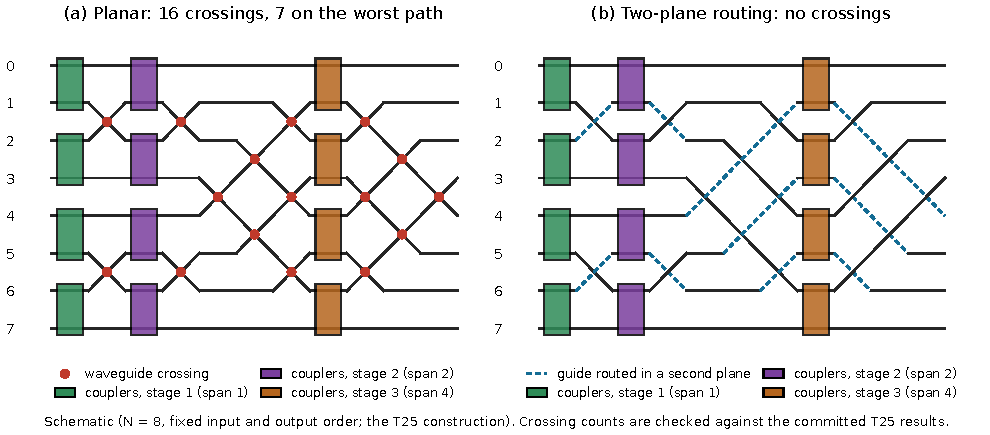
\includegraphics[width=0.94\linewidth]{figures/fig_layout_schematic.pdf}
\caption{Schematic of the planar and two-plane routing of an 8-mode butterfly (model construction, not a fabricated layout). (a) The T25 layout with fixed input and output order: adjacent swaps (red dots, one waveguide crossing each) interleave the partners before each coupler stage and restore the order afterwards; 16 crossings in total and 7 on the worst light path, equal to the committed T25 counts. (b) The same network with the guides of one block routed in a second plane (dashed): no physical crossings, at the price of out-of-plane transitions whose loss is the open question of Section~\ref{sec:t25}. This drawing is one illustrative 3D routing; the T25 loss model assigns one vertical-transition loss per stage.}
\label{fig:schematic}
\end{figure}

\subsection{Energy model of a passive optical layer}
\label{sec:energymodel}

The budget (\texttt{agentkit.limits.layer\_budget}) describes a dense passive layer with $N$ inputs and $M$ outputs, $b$ bits of output precision and sample rate $f_s$ ($T=1/f_s$). Each detector integrates $\Ne$ photoelectrons per sample with shot noise and the thermal noise of its transimpedance amplifier,
\begin{equation}
\sigma^2=\Ne+\sigma_\mathrm{th}^2,\qquad \sigma_\mathrm{th}=\frac{i_n\sqrt{B}\,T}{q},\qquad B=\frac{f_s}{2},
\label{eq:noise}
\end{equation}
where $i_n$ is the input-referred noise current density and $q$ the elementary charge. Resolving $L=2^b$ levels at $k$ standard deviations per half level ($k=1$ in the registered test) requires $k\sigma\le\Ne/(2L)$, whose solution is
\begin{equation}
\Ne=2k^2L^2\left[1+\sqrt{1+\frac{\sigma_\mathrm{th}^2}{k^2L^2}}\right].
\label{eq:ne}
\end{equation}
With quantum efficiency $\eta$, each detector needs $N_\mathrm{ph}=\Ne/\eta$ photons, an optical energy $E_\mathrm{det}=N_\mathrm{ph}hc/\lambda$ per sample. The laser, with wall-plug efficiency $\eta_\mathrm{wp}$, must supply this energy to all $M$ detectors through a total optical transmission $T_\mathrm{opt}$, so the energy per frame of $NM$ MACs is
\begin{equation}
E_\mathrm{frame}=\frac{M\,E_\mathrm{det}}{T_\mathrm{opt}\,\eta_\mathrm{wp}}+N\,(E_\mathrm{mod}+E_\mathrm{DAC})+M\,E_\mathrm{ADC}+\frac{P_\mathrm{static}}{f_s},
\qquad E_\mathrm{MAC}=\frac{E_\mathrm{frame}}{NM},
\label{eq:frame}
\end{equation}
with modulator-plus-driver, digital-to-analog and analog-to-digital converter energies per sample $E_\mathrm{mod}$, $E_\mathrm{DAC}$, $E_\mathrm{ADC}$ and static power $P_\mathrm{static}$. The advantage factor against a digital reference is $A=E_\mathrm{ref}/E_\mathrm{MAC}$. The transmission collects every loss in decibels,
\begin{equation}
-10\log_{10}T_\mathrm{opt}=2L_\mathrm{facet}+(2\,\mathrm{cm})\,\alpha_\mathrm{prop}+L_\mathrm{mod}+2N\ell_\mathrm{s},
\label{eq:transmission}
\end{equation}
where the last term is the mesh of the SVD realization (Section~\ref{sec:synthesis}). For a square layer ($N=M$) the electronic terms give a floor that does not depend on the optical core,
\begin{equation}
E_\mathrm{conv}=\frac{E_\mathrm{mod}+E_\mathrm{DAC}+E_\mathrm{ADC}}{N},
\label{eq:floor}
\end{equation}
which falls only as $1/N$. Finally, the laser power $P_\mathrm{las}$ limits the depth of a cascade: the largest number of stages that still leaves $E_\mathrm{det}$ at every detector is
\begin{equation}
S_\mathrm{max}=\left\lfloor\frac{10\log_{10}\!\left[P_\mathrm{las}/(f_s\,M\,E_\mathrm{det})\right]-L_\mathrm{fixed}}{\ell_\mathrm{s}}\right\rfloor,\qquad L_\mathrm{fixed}=2L_\mathrm{facet}+L_\mathrm{mod}.
\label{eq:maxdepth}
\end{equation}
The protocol fixed the registered point ($N=M=64$, $b=8$, $f_s=1$\,GS/s, $k=1$), a sensitivity grid ($N\in\{16,64,256\}$, $b\in\{4,6,8\}$, $f_s\in\{1,10\}$\,GS/s), the parameter-selection rules (nominal: typical value from a primary source for commercially available or routinely demonstrated components at 1550\,nm, 2015--2026; optimistic: best peer-reviewed demonstrated value), the two digital references and the decision rule, all before any value was gathered. A programmable variant, reported for information only, adds the mean power of two thermo-optic shifters per MZI.

\subsection{Splitter-error and calibration model}
\label{sec:calmodel}

Each coupler of a simulated Clements mesh has a splitting-angle error $\varepsilon=\varepsilon_\mathrm{sh}+\varepsilon_{\mathrm{loc},k}$, with a component $\varepsilon_\mathrm{sh}\sim\mathcal N(0,\rho\sigma^2)$ shared by all couplers of a device (as for a common writing bias) and independent local components $\varepsilon_{\mathrm{loc},k}\sim\mathcal N(0,(1-\rho)\sigma^2)$; $\rho$ is the shared fraction of the variance. The figure of merit is the global-phase-insensitive infidelity
\begin{equation}
\mathcal I=1-\frac{|\mathrm{Tr}(U^\dagger V)|}{N}
\label{eq:infidelity}
\end{equation}
between the target $U$ and the realized $V$. Four strategies are compared on Haar-random targets (a new target per realization): (A) phases computed for an error-free mesh; (B) all $2\cdot N(N-1)/2+N$ phases re-optimized on the erroneous device with exact access to its transfer matrix, by L-BFGS-B from A with an exact analytic gradient (at most 1000 iterations); (B, 8-bit) the phases of B rounded to an 8-bit DAC over $2\pi$; and (C) phases optimized on a model whose splitter errors were characterized with an error of standard deviation $0.1\sigma$, then applied to the true device. Tail statements use the 95/95 Wilks bound of Section~\ref{sec:integrity}. The same error model, without calibration, is used in T25 to compare the DFT realized by a Clements mesh and by a butterfly through the fidelity $1-\mathcal I$.

%======================================================================
\section{Results}
\label{sec:results}

\subsection{Earlier results carried into the closure}
\label{sec:prior}

Table~\ref{tab:prior} summarizes the earlier numerical results on which the kill tests build, with their registered status, and Table~\ref{tab:vector} the vector modes of the trench guide. Two points matter for what follows. The HE$_{11}$ leakage of the $t=12$\um trench, 0.044\dBcm, is the floor of the waveguide hypothesis H1 (Section~\ref{sec:nexttest}); the higher-order modes leak at 2.75--2.79\dBcm. Several earlier hypotheses failed their registered criteria and are kept as negative or partial results.

\begin{table}[t]
\centering\small
\caption{Earlier numerical results and their registered status (details, evidence paths and hashes in Table~\ref{tab:claims}). All are models; none is a measurement.}
\label{tab:prior}
\begin{tabularx}{\linewidth}{>{\raggedright\arraybackslash}p{3.7cm}X>{\raggedright\arraybackslash}p{2.6cm}}
\toprule
Item & Result & Status \\
\midrule
Vector leakage of the trench guide & HE$_{11}$: $n_\mathrm{eff}=1.442189$, leakage 0.044\dBcm; TE$_{01}$/TM$_{01}$: 2.75--2.79\dBcm & model (layer solver) \\
Scalar versus vector & TE/TM splitting $\sim3\times10^{-6}$; scalar finite differences reach $4.2\times10^{-6}$ at $h=0.125$\um (order 1.4) and cannot resolve it & partial (T06) \\
Paraxial BPM loss artefact & guided-mode loss $2.8\times10^{-8}$ and $2.7\times10^{-8}$\,mm$^{-1}$ at $\Delta z=0.125$ and 0.0625\um; artefact for $\Delta z\ge0.25$\um & partial \\
Time convergence of the D16 model & two audits passed; the fine run F1 stopped at 96 of 192 fields and its outputs were not recovered; a replacement run (F1R) was preregistered on 13 October 2026, and no result of it is reported here & open (T01) \\
Calibration-aware compiler & C1 met; C2 failed ($1.3$--$1.7\times10^{-2}$ against $5\times10^{-3}$); C3 met in 28 of 36 realizations (77.8\,\%, exact 95\,\% CI 60.8--89.9\,\%) & partial (T11) \\
Correlated phase errors & H10b failed: a correlation length raised the 95th percentile by a factor 1.68 (registered band 0.8--1.25) & partial (T10) \\
Small optoelectronic network F3-b & 64.25\,\% test accuracy against 84.55\,\% for a non-converged electronic reference; majority class 52.5\,\% & registered negative (T12) \\
Graphics-pipeline field rendering & R1, R2 and P1 failed precision; R3 rendered 84 of 84 analytic fields per backend within $5.9\times10^{-7}$ (representation only, not propagation) & mixed \\
\bottomrule
\end{tabularx}
\end{table}

\subsection{T25: depth and crossings of planar and three-dimensional meshes}
\label{sec:t25}

\emph{Question.} Can writing in three dimensions reduce the depth, the crossings or the error accumulation of a photonic mesh? The seven registered criteria are computational verification gates (depth of both syntheses, reconstruction error, closed form, dynamic programme against brute force, DFT factorization error, depth bound respected); all seven were met in the amended run (Table~\ref{tab:protocols}). Figure~\ref{fig:t25} summarizes the results.

\paragraph{Depth.} For every $N$ from 3 to 16 the rectangular synthesis has depth $N$ and the triangular synthesis $2N-3$, with a largest reconstruction error of $3.8\times10^{-15}$ (Table~\ref{tab:depth}). Together with Proposition~\ref{prop:depth}, \textbf{three-dimensional connectivity can save at most one layer} of a universal mesh: one for even $N$, none for odd $N$. The first wording of this result in the project, ``3D cannot reduce the logical depth'', was false by up to one layer and was corrected after the review (Section~\ref{sec:review}). Any 3D advantage must therefore come from crossings, density, routing length or structured, non-universal transforms.

\begin{table}[t]
\centering\small
\caption{Depth of universal meshes (T25, ideal transfer algebra). The lower bound is that of Proposition~\ref{prop:depth}; the T25 run used $N-1$ for all $N$, which is the bound for even $N$.}
\label{tab:depth}
\begin{tabular}{@{}rccccc@{}}
\toprule
$N$ & Lower bound & Rectangular depth & Triangular depth & MZIs & Couplers \\
 & (Prop.~\ref{prop:depth}) & (synthesized) & (synthesized) & $N(N-1)/2$ & \\
\midrule
3 & 3 & 3 & 3 & 3 & 6 \\
4 & 3 & 4 & 5 & 6 & 12 \\
8 & 7 & 8 & 13 & 28 & 56 \\
16 & 15 & 16 & 29 & 120 & 240 \\
\bottomrule
\end{tabular}
\end{table}

\paragraph{Crossings.} Table~\ref{tab:crossings} gives the counts of the planar butterfly. The total follows Eq.~\eqref{eq:crossings} for every $N$; the worst path crosses 2, 7, 18, 41 and 88 guides for $N=4$, 8, 16, 32 and 64 with fixed order, and 4, 11, 26 and at most 57 for $N=8$, 16, 32 and 64 with free output order. The break-even crossing loss at $N=16$ is 0.022\dB per crossing with fixed order and 0.036\dB with free output order.

\begin{table}[t]
\centering\small
\caption{Crossings of a planar radix-2 butterfly (T25 and review recomputation; model). Break-even: per-crossing loss at which the worst-path planar penalty equals $2U=0.4$\dB.}
\label{tab:crossings}
\begin{tabular}{@{}rrrrrrr@{}}
\toprule
 & & \multicolumn{3}{c}{Fixed input and output order} & \multicolumn{2}{c}{Free output order} \\
\cmidrule(lr){3-5}\cmidrule(lr){6-7}
$N$ & Couplers & Total & Worst path & Break-even (dB) & Total & Worst path \\
\midrule
4 & 4 & 2 & 2 & 0.200 & -- & -- \\
8 & 12 & 16 & 7 & 0.057 & 8 & 4 \\
16 & 32 & 88 & 18 & 0.022 & 44 & 11 \\
32 & 80 & 416 & 41 & 0.0098 & 208 & 26 \\
64 & 192 & 1824 & 88 & 0.0045 & 912 & $\le57$ \\
128 & 448 & 7680 & 183 & 0.0022 & -- & -- \\
256 & 1024 & 31616 & 374 & 0.0011 & -- & -- \\
\bottomrule
\end{tabular}
\end{table}

\paragraph{Worst-path loss.} On the grid of Eq.~\eqref{eq:pathloss} (stage loss 0.1\dB and vertical transition 0.05\dB per stage), at $N=16$ the planar Clements mesh has 1.60\dB, the planar butterfly 0.76\dB at 0.02\dB per crossing and 2.20\dB at 0.10\dB, and the 3D butterfly 0.60\dB; at $N=64$ the values are 6.40, 2.36, 9.40 and 0.90\dB. Against a planar Clements mesh (rule I3), the 3D butterfly saves $N-\log_2N$ stages, 12 at $N=16$ and 58 at $N=64$ (1.2 and 5.8\dB at 0.1\dB per stage), at the cost of universality. The vertical-transition grid (0--0.1\dB per stage) is optimistic: the only source of a verified crossing loss reports 0.4--0.5\dB per S-bend at a 50\,mm radius \cite{Djogo2026}.

\paragraph{Rule I1 applied.} The registered rule takes the lowest verified per-crossing loss $\ell_\mathrm{x}$ from T26, here at most 0.01\dB (Section~\ref{sec:t26}). It is below the break-even loss at $N=16$, so the crossing advantage is not measurable at that size, and the rule asks for the smallest $N$ with $X(N)\,\ell_\mathrm{x}\ge2U$. With the fixed-order layout this is $N=32$ ($41\times0.01=0.41$\dB); with free output order it is $N=64$ ($57\times0.01=0.57$\dB, against $26\times0.01=0.26$\dB at $N=32$), at the edge of the rule, which withdraws the crossing argument as a headline if that $N$ exceeds 64. Because 0.01\dB is an upper bound measured at 80$^\circ$, the true threshold may be larger, and the comparison ignores the S-bends on both sides. The crossing argument is therefore retained only for structured transforms with $N\ge64$, as a secondary hypothesis, and it has a 2016 precedent \cite{Crespi2016}.

\paragraph{Error accumulation.} With uncalibrated splitter errors of 0.02\,rad (rule I2, descriptive), the butterfly DFT, with far fewer couplers, keeps higher fidelity than the Clements DFT (Table~\ref{tab:errors}); at $N=16$ the 5th percentiles are 0.99885 and 0.99226 without a shared component. A shared component barely changes the means but widens the lower tail of both. The butterfly is not universal, so this compares different function classes and applies only to tasks that need a structured transform; the percentiles are descriptive statistics of the model, not tolerance bounds for fabricated parts.

\begin{table}[t]
\centering\small
\caption{DFT fidelity $|\mathrm{Tr}(U^\dagger V)|/N$ under splitter-angle errors $\sigma=0.02$\,rad, 200 realizations, no calibration (T25, model).}
\label{tab:errors}
\begin{tabular}{@{}rcrrcc@{}}
\toprule
$N$ & Shared fraction $\rho$ & \multicolumn{2}{c}{Couplers} & Clements mean / 5th pct. & Butterfly mean / 5th pct. \\
 & & Clements & Butterfly & & \\
\midrule
4 & 0.0 & 12 & 4 & 0.99879 / 0.99766 & 0.99960 / 0.99912 \\
4 & 0.8 & 12 & 4 & 0.99888 / 0.99623 & 0.99960 / 0.99866 \\
8 & 0.0 & 56 & 12 & 0.99717 / 0.99575 & 0.99940 / 0.99898 \\
8 & 0.8 & 56 & 12 & 0.99803 / 0.99386 & 0.99942 / 0.99801 \\
16 & 0.0 & 240 & 32 & 0.99404 / 0.99226 & 0.99920 / 0.99885 \\
16 & 0.8 & 240 & 32 & 0.99686 / 0.99110 & 0.99920 / 0.99757 \\
\bottomrule
\end{tabular}
\end{table}

\begin{figure}[t]
\centering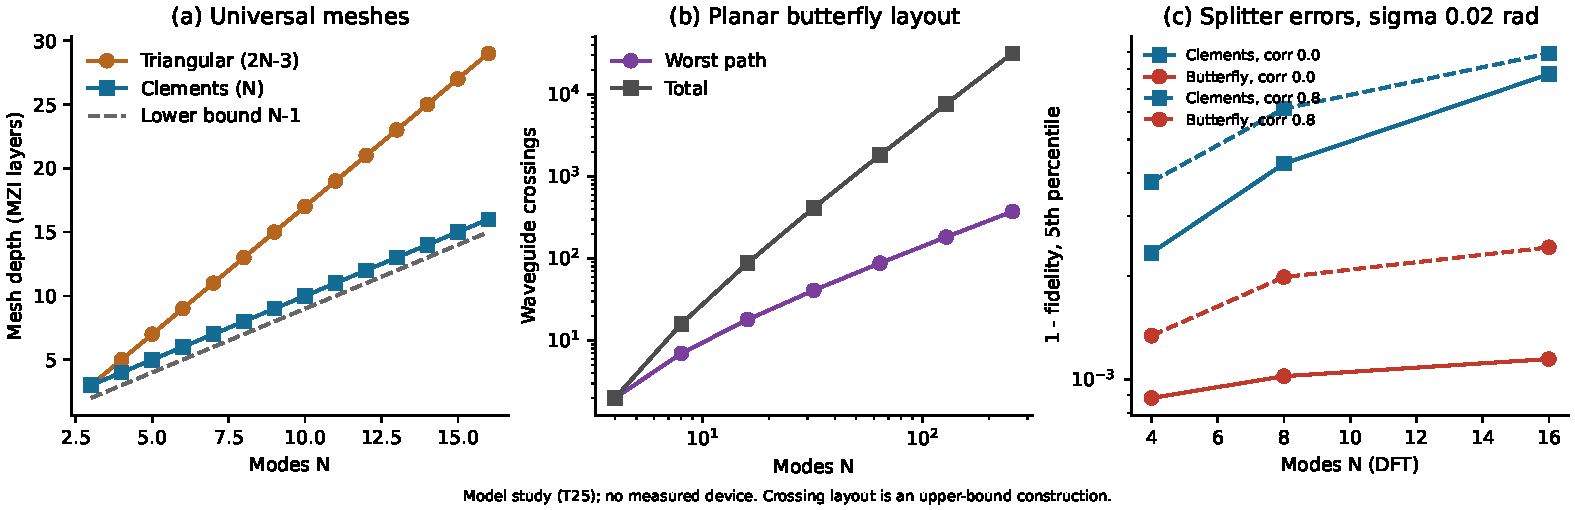
\includegraphics[width=0.94\linewidth]{figures/fig_t25_scaling.pdf}
\caption{T25 (model; no measured device). (a) Depth of universal meshes; the dashed line is the bound $N-1$, valid for even $N$ (for odd $N$ the bound of Proposition~\ref{prop:depth} is $N$). (b) Total and worst-path crossings of the planar butterfly layout with fixed input and output order; freeing the output order halves the total (Table~\ref{tab:crossings}). (c) 5th-percentile infidelity of the DFT under splitter errors, Clements versus butterfly, without and with a shared error component (corr = $\rho$).}
\label{fig:t25}
\end{figure}

\subsection{T27: in-situ recalibration of fabrication errors}
\label{sec:t27}

\emph{Question.} Couplers written by fs laser have fabrication errors, partly shared across a chip. Can in-situ recalibration of a programmable mesh absorb them? The registered criteria at the primary point ($N=8$, $\sigma=0.02$\,rad, $\rho=0.8$, 60 Haar targets) were a gradient check with relative error at most $10^{-6}$, a 95/95 upper bound of the infidelity after calibration of at most $10^{-3}$, and a median improvement factor of at least 10. All three were met (Table~\ref{tab:t27primary}, Fig.~\ref{fig:t27}): the gradient check gave $2.7\times10^{-9}$ and the bound $1.32\times10^{-4}$. The run took 1056\,s on one CPU thread.

\begin{table}[t]
\centering\small
\caption{T27 primary point: $N=8$, $\sigma=0.02$\,rad, shared fraction 0.8, 60 realizations (model).}
\label{tab:t27primary}
\begin{tabular}{@{}lcc@{}}
\toprule
Strategy & Median infidelity & 95/95 upper bound \\
\midrule
A, ideal programming & $1.6\times10^{-3}$ & $1.5\times10^{-2}$ \\
B, in situ & $5\times10^{-14}$ & $1.3\times10^{-4}$ \\
B, 8-bit DAC & $1.8\times10^{-4}$ & $3.7\times10^{-4}$ \\
C, model-based ($0.1\sigma$ characterization error) & $2.7\times10^{-5}$ & $1.6\times10^{-4}$ \\
\bottomrule
\end{tabular}
\end{table}

The median improvement factor, $3.1\times10^{10}$, is dominated by post-calibration values at machine precision and should not be read as a physical ratio; the medians and bounds carry the result. In 55 of the 60 realizations the in-situ infidelity is below $10^{-6}$. In the other five ($5.0\times10^{-6}$ to $1.3\times10^{-4}$) the erroneous couplers cannot reach the target exactly, and one of these five optimizations stopped at the iteration limit (two of the 60 did, the other reaching $6.7\times10^{-13}$). The 8-bit phase DAC sets a floor of about $2\times10^{-4}$ in median infidelity at $N=8$, so reaching $10^{-4}$ needs finer phase control. Model-based precompensation with a characterization error of $0.1\sigma$ comes close to the in-situ bound but not to its median.

On the secondary grid (Table~\ref{tab:t27grid}), calibration absorbs splitter errors of 0.02\,rad almost completely for $N=4$ and 8, correlated or not. A shared component is harder for uncalibrated meshes ($1.7\times10^{-2}$ against $4.2\times10^{-3}$ at $N=8$, $\sigma=0.02$\,rad) but is removed by calibration. At $\sigma=0.05$\,rad with independent errors and $N=8$ the $10^{-3}$ level is not reached ($2.3\times10^{-3}$): larger errors make more targets unreachable for a Clements mesh, and error-tolerant architectures \cite{Saygin2020,Kondratyev2024} are the alternative to test. The model omits thermal crosstalk, drift, loss and measurement noise, assumes exact access to the device transfer matrix and applies only to programmable meshes; a fixed, written mesh cannot be recalibrated, and for it only strategy C applies. The support for the calibration hypothesis H-C is therefore limited to $N\le8$, $\sigma\le0.02$\,rad and ideal access; the next model tests are $N=16$ and 32 and an intensity-only, noisy calibration loop.

\begin{figure}[t]
\centering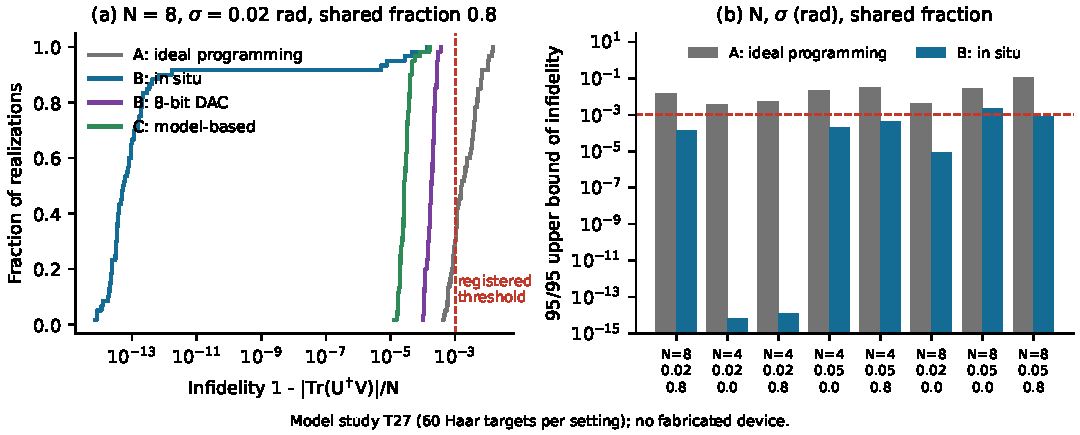
\includegraphics[width=0.9\linewidth]{figures/fig_t27_calibration.pdf}
\caption{T27 (model; no fabricated device). (a) Distribution of the infidelity at the primary point for ideal programming, in-situ calibration, 8-bit quantization and model-based precompensation. (b) 95/95 upper bounds before and after calibration on the primary point and the secondary grid; the dashed line is the registered threshold.}
\label{fig:t27}
\end{figure}

\subsection{T24: energy per multiply--accumulate}
\label{sec:t24}

\emph{Question.} Could a passive optical layer in glass, with all its electronics, need less energy per MAC than a digital reference at equal 8-bit precision (hypothesis H-A)? The protocol, committed and verified on the server before any value was gathered, fixed the model of Section~\ref{sec:energymodel}, the registered point, the selection rules, two digital references and the decision rule. Component values were then collected under the frozen rules, their 22 DOIs were checked against Crossref for title and year, and the parameter files were frozen and published before the budget was computed. The parameters and their sources are in Table~\ref{tab:params} (Appendix~\ref{app:params}). The digital references are 0.23\,pJ per MAC for 8-bit arithmetic at 45\,nm in 2014 (0.2\,pJ multiply plus 0.03\,pJ add, arithmetic only, lenient to optics) \cite{Horowitz2014} and 16.05\fJ per MAC for a 3\,nm INT8 digital compute-in-memory macro in 2026 (124.6\,TOPS/W at 0.5\,V, two operations per MAC, macro level, strict for optics) \cite{Mori2026}. The decision rule discards H-A if the optimistic advantage against the 2014 reference is at most 1, and withdraws it as a headline if the optimistic advantage against the modern reference is below 1; the registered criterion is the latter.

\paragraph{The robust part: a converter floor.} At the registered point the DACs, ADCs and modulators alone cost, per MAC, 72.9, 83.5 and 18.3\fJ with the nominal values and 49.1, 17.4 and 5.2\fJ with the optimistic ones (Table~\ref{tab:t24}). By Eq.~\eqref{eq:floor} their sum, 71.6\fJ per MAC with the optimistic values, does not depend on the optical core: it is 4.5 times the 3\,nm macro at 0.5\,V. The review estimated that at nominal supply voltage the macro needs about three times more energy, about 0.05\,pJ per MAC; against that value the margin shrinks to about 1.4. The comparison with modern digital hardware is therefore lost at $N=64$ even for a lossless optical core. The exploratory lossless case of the optimistic set gives 75.0\fJ per MAC (advantage 0.21 against the 3\,nm macro), and break-even with that macro would need $N\approx300$ even without mesh loss (Fig.~\ref{fig:t24}b), a size whose mesh would be hundreds of decibels long at present stage losses. Against the 2014 reference the converters alone do not lose: the deciding term is the mesh.

\begin{table}[t]
\centering\small
\caption{T24 budget at the registered point ($N=M=64$, 8 bits, 1\,GS/s, $k=1$; parametric budget from cited values, not a measurement). Energies per MAC unless stated.}
\label{tab:t24}
\begin{tabular}{@{}>{\raggedright\arraybackslash}p{6.2cm}cc@{}}
\toprule
 & Nominal & Optimistic \\
\midrule
Laser (electrical) & 1.20\,nJ & 0.10\,nJ \\
DAC / ADC / modulator & 72.9 / 83.5 / 18.3\fJ & 49.1 / 17.4 / 5.2\fJ \\
Converters plus modulators, Eq.~\eqref{eq:floor} & 174.7\fJ & 71.6\fJ \\
Static & 0.29\,pJ (1.2\,W) & 0 (assumption) \\
Total & 1.2\,nJ & 0.10\,nJ \\
Thermal noise $\sigma_\mathrm{th}$ (electrons) & 1396 & 279 \\
Photons per detector and sample & $1.13\times10^{6}$ & $3.53\times10^{5}$ \\
Optical transmission & $-47.3$\dB & $-46.3$\dB \\
Advantage against 3\,nm INT8 (2026) & $1.3\times10^{-5}$ & $1.6\times10^{-4}$ \\
Advantage against 45\,nm (2014) & $1.9\times10^{-4}$ & $2.3\times10^{-3}$ \\
Stages allowed by laser power / needed ($2N+1$) & 22 / 129 & 77 / 129 \\
Programmable variant: static power, 4032 heaters & 128.2\,W (air) & 1.45\,W (vacuum) \\
\bottomrule
\end{tabular}
\end{table}

\paragraph{The fragile part: the mesh.} The totals are 1.2\,nJ (nominal) and 0.10\,nJ (optimistic) per MAC, dominated by the laser. A general passive layer realized by singular-value decomposition needs two universal meshes, $2N=128$ MZI layers at 0.35\dB each \cite{Ceccarelli2020}, 44.8\dB of mesh loss, which multiplies the required laser energy by about $3\times10^4$; the $2N+1=129$ layers exceed the 22 (nominal) or 77 (optimistic) stages that the laser power can feed (Eq.~\eqref{eq:maxdepth}). The advantage factors are $1.3\times10^{-5}$ and $1.6\times10^{-4}$ against the 3\,nm macro and $1.9\times10^{-4}$ and $2.3\times10^{-3}$ against the 45\,nm MAC. The registered criterion (optimistic advantage against the modern reference at least 1) is not met; the other two criteria (all parameters sourced, all DOIs verified) are met. By the registered rule H-A is discarded and kept as a registered negative; the ledger records it as withdrawn for the robust reason (claim C-HA-energy). No point of the registered sensitivity grid (36 points) reaches an advantage of 1; the largest values, 0.057 against the modern and 0.82 against the 2014 reference, occur for the optimistic set at $N=256$, 4 bits and 10\,GS/s. The registered sweep keeps the $N=64$ mesh transmission for every $N$, so it is optimistic for $N>64$ and pessimistic for $N<64$.

\paragraph{Researcher degrees of freedom.} Three choices were made after the commitment, all against H-A: the SVD realization of the layer (the protocol says only ``mesh excess loss''), the optimistic stage loss set equal to the nominal one, because the only per-MZI value found for fs-written glass is 0.35\dB in EAGLE XG borosilicate \cite{Ceccarelli2020}, and single-mode laser values, because a coherent mesh needs a single-mode source (the multimode values found, 50\,\% wall-plug efficiency and 4.9\,W \cite{Garrod2014,Kanold2024}, are recorded but not used, and would not change the verdict). Conversely, the optimistic set is lenient on electronics: $k=1$ at half an LSB, a binary (NRZ) modulator energy used for an 8-bit analog modulator, an ADC of effective resolution about 7.3 bits and no static power. With these choices the verdict against the 2014 reference is fragile. A stage loss of at most 0.131\dB (mesh at most 16.7\dB) would reverse it; 0.07\dB per stage, the loss of a 1.2\,cm MZI at the 0.06\dBcm of Section~\ref{sec:t26}, gives 98\fJ per MAC, 2.3 times better than the 2014 MAC and 6 times worse than the 3\,nm macro; an illustrative fan-out realization with about 12 stages gives about 80\fJ per MAC. These sensitivities were computed after the commitment and are not part of the registered test.

\paragraph{Programmable meshes.} Thermo-optic programmability adds static power: one $64\times64$ Clements mesh has 4032 shifters (the two-mesh SVD layer of the budget has twice as many), which at a mean 31.5\,mW each \cite{Pentangelo2024} draw 127\,W in air. Only vacuum-packaged shifters (mean 0.36\,mW \cite{Ceccarelli2020}) bring this to about 1.5\,W. The budget per MAC excludes memory traffic on both sides, and several values were read from abstracts or datasheets by search agents (flagged in the raw search file); none of them changes the verdict by orders of magnitude.

\begin{figure}[t]
\centering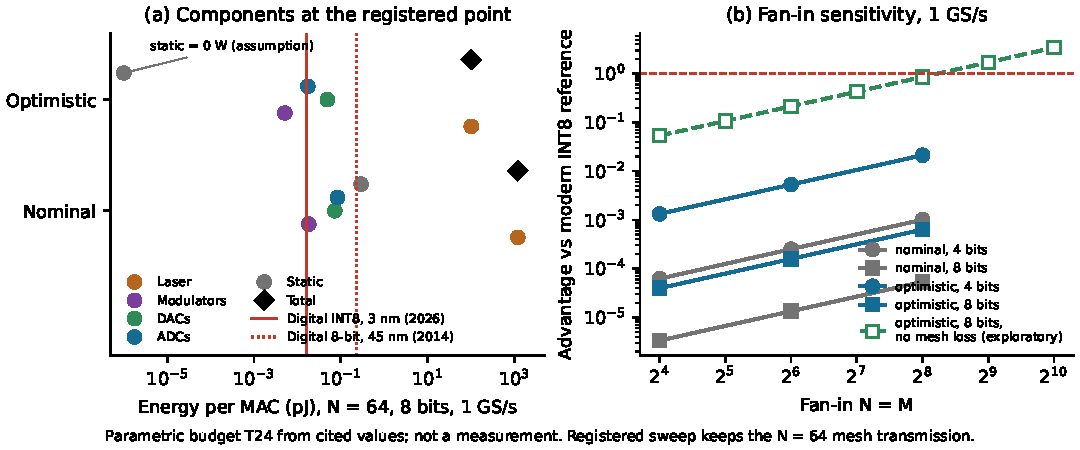
\includegraphics[width=0.9\linewidth]{figures/fig_t24_energy.pdf}
\caption{T24 (parametric budget from cited values; not a measurement). (a) Energy per MAC by component at the registered point for the nominal and optimistic sets, with the two digital references; the static term of the optimistic set is zero by assumption and drawn at the axis floor. (b) Advantage factor against the 3\,nm INT8 reference versus fan-in. The registered sweep keeps the $N=64$ mesh transmission; the dashed curve is an exploratory optimistic case without mesh loss.}
\label{fig:t24}
\end{figure}

\subsection{T26: state of the art for the waveguide and crossing hypotheses}
\label{sec:t26}

\emph{Question.} Against which verified results must the project's waveguide hypothesis H1 and its crossing argument H-B be judged? A separate search agent followed a frozen strategy (date window 2010 to 12 October 2026; Crossref, arXiv, publisher pages and one level of snowballing). It logged 41 queries and included 31 records; all 31 identifiers were verified against Crossref or arXiv, every extracted value records where it appears in the source, and the registered criteria (all identifiers verified, at least 8 verified records, every value located) were met. The two values that decide the registered rules were then re-read by a second reader in the primary text. Twelve documented gaps record what could not be verified. Figure~\ref{fig:sota} shows the 16 records that report both a loss and a wavelength.

\paragraph{Rule R1: propagation loss at 1530--1565\,nm in fused silica.} The lowest verified value is $0.06\pm0.02$\dBcm for a single-mode multiscan guide written with UV (343\,nm, 450\,fs) pulses, by cut-back from 13 to 2.5\,cm with light at 1550\,nm butt-coupled from a standard single-mode fibre \cite{Ackermann2025}; after annealing the same work reports $0.02\pm0.04$\dBcm, an uncertainty larger than the value. Because this is below the 0.3\dBcm threshold of H1, rule R1 relabels that threshold as a feasibility threshold and registers a secondary hypothesis, H1-SOTA, with threshold 0.06\dBcm under the same three-zone rule. The H1 threshold itself came from a tubular guide in fused silica \cite{Bukharin2015} whose abstract gives no wavelength.

\paragraph{Rule R3: depressed-cladding guides at 1530--1565\,nm.} No verified record was found. Bukharin et al.\ \cite{Bukharin2015} give no wavelength in the abstract, Likhov et al.\ \cite{Likhov2025} state 0.8\dBcm in K8 glass for the ``telecom range'', and the 2025 study of telecom-band depressed-cladding guides in SK1310 glass \cite{Zhou2025} has no abstract in Crossref or Semantic Scholar and its publisher page could not be read. This is a gap in what we could verify, not evidence that no such measurement exists; that study very likely reports telecom-band losses and must be read before any priority statement.

\paragraph{Rule R4: crossings.} The only verified per-crossing figure is an upper bound: at most 0.01\dB per crossing at 80$^\circ$ in fused silica at 1550\,nm, with up to 16 crossings and crosstalk below a 40\dB noise floor \cite{Djogo2026}. No data were found for 90$^\circ$ or shallow angles, which are those of the swaps of a planar butterfly, nor a per-crossing value for fs-written 3D overpasses. This value feeds rule I1 (Section~\ref{sec:t25}).

\paragraph{Rule R5: networks.} Programmable fs-written meshes at 1550\,nm \cite{Pentangelo2024}, error-tolerant designs \cite{Kondratyev2024}, crossing-free 3D Fourier circuits \cite{Crespi2016}, large 3D continuously coupled circuits \cite{Hoch2022,DiMicco2026}, a 24-mode universal processor \cite{Barzaghi2025} and a 3D multilayer neural network in glass \cite{Cao2026} all have precedents. A multilayer 3D fs-written network in glass is therefore not new, and the ledger withdraws the project's claim that it was (C-T19-a, because of \cite{Cao2026}); the claim of a first fs-written depressed-cladding trench guide at 1550\,nm is withdrawn as well (C-T19-c, because of \cite{Zhou2025}). The crossing argument for 3D routing has a 2016 precedent \cite{Crespi2016} and carries no novelty.

\begin{figure}[t]
\centering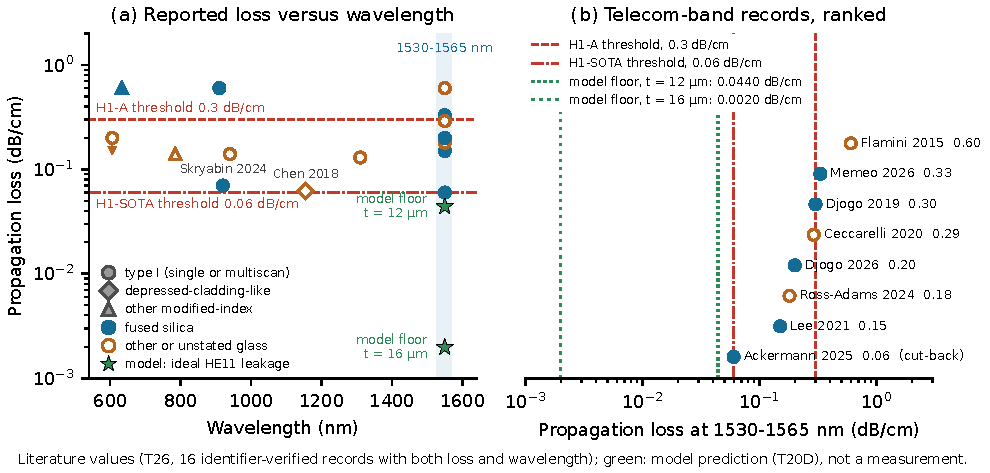
\includegraphics[width=\linewidth]{figures/fig_sota_loss.pdf}
\caption{State of the art (literature, T26) and the predicted leakage floors (model, T20D). (a) Propagation loss versus wavelength for the 16 identifier-verified records that report both quantities; marker shape gives the waveguide type and filling the glass (filled: fused silica). The arrow marks a value reported as an upper bound. The shaded band is 1530--1565\,nm, the dashed and dash-dotted lines are the H1-A and H1-SOTA thresholds, and the stars are the ideal HE$_{11}$ leakage floors of the project's trench guide at $t=12$ and 16\um. (b) The eight records in the telecom band, ranked, against the same thresholds and floors. Tan et al.\ 2022 (0.07\dBcm) is not plotted because its wavelength is not verified.}
\label{fig:sota}
\end{figure}

\subsection{T20D: trench width for a state-of-the-art test}
\label{sec:t20d}

\emph{Question.} How wide must the trench be for the ideal HE$_{11}$ leakage floor to stay at or below 10\,\% of the verified state of the art, that is at most 0.006\dBcm? With $t=12$\um the floor is 0.044\dBcm, so H1-SOTA could only be confirmed if the whole 95\,\% interval lay within $[0.044,0.06]$\dBcm, an interval narrower than 0.016\dBcm that would also leave only 0.016\dBcm for scattering and absorption. That is not a sensible test. The design study T20D was therefore registered before any fabrication or measurement, with a grid of widths, three verification criteria and a decision rule: $t_\mathrm{min}$ is the smallest width, by log-linear interpolation, with leakage at most 0.006\dBcm, and the H1-SOTA coupon uses the next whole micrometre above $t_\mathrm{min}$ plus 1\um of margin. Before the commitment, one solve at $t=12$\um reproduced the registered value to check the solver and its run time; no other width was computed.

\begin{table}[t]
\centering\small
\caption{T20D: HE$_{11}$ of the trench guide versus trench width ($\Delta n=-0.005$, $a=6$\um, $n_0=1.444$, $\lambda=1550$\,nm; exact vector solver, model).}
\label{tab:t20d}
\begin{tabular}{@{}rccc@{}}
\toprule
$t$ (\textmu m) & Re\,$n_\mathrm{eff}$ & Im\,$n_\mathrm{eff}$ & Leakage (dB/cm) \\
\midrule
12 & 1.442189333 & $1.25\times10^{-7}$ & 0.0440 \\
13 & 1.442189314 & $5.76\times10^{-8}$ & 0.0203 \\
14 & 1.442189305 & $2.65\times10^{-8}$ & 0.0093 \\
15 & 1.442189301 & $1.22\times10^{-8}$ & 0.0043 \\
16 & 1.442189299 & $5.62\times10^{-9}$ & 0.0020 \\
18 & 1.442189298 & $1.19\times10^{-9}$ & 0.00042 \\
20 & 1.442189297 & $2.52\times10^{-10}$ & 0.000089 \\
\bottomrule
\end{tabular}
\end{table}

All seven solves were valid, the leakage decreases monotonically with width, and the $t=12$\um value reproduces the registered one, so all three criteria were met (Table~\ref{tab:t20d}, Fig.~\ref{fig:trench}). The leakage falls by roughly a factor of two per micrometre of trench, while the real part of the index changes only in the eighth decimal. Interpolating between 14 and 15\um gives $t_\mathrm{min}=14.57$\um, so the registered rule sets the H1-SOTA coupon at $t=16$\um, whose ideal floor is 0.0020\dBcm (0.00198\dBcm), about 3\,\% of the state of the art. A cut-back of that guide would measure scattering and absorption against the state of the art rather than leakage. The run took 987\,s on one CPU thread and started about 40\,s after the commitment was recorded; the review confirmed the order of events (Table~\ref{tab:timeline}).

\begin{figure}[t]
\centering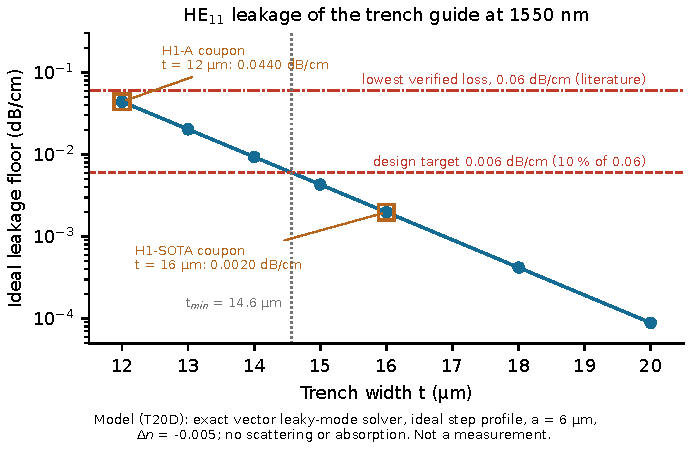
\includegraphics[width=0.66\linewidth]{figures/fig_trench_leakage.pdf}
\caption{T20D (model; not a measurement). Ideal HE$_{11}$ leakage floor of the trench guide versus trench width, from the exact vector leaky-mode solver (log scale; straight segments are the log-linear interpolation of the decision rule). Dashed: design target 0.006\dBcm; dash-dotted: lowest verified loss at 1550\,nm (literature, 0.06\dBcm). Squares: the H1-A coupon ($t=12$\um) and the H1-SOTA coupon ($t=16$\um); dotted: $t_\mathrm{min}=14.6$\um.}
\label{fig:trench}
\end{figure}

%======================================================================
\section{Adversarial review and what it changed}
\label{sec:review}

After the four tests and the first choice of a central claim, a separate agent (Claude Opus), with read-only access and no authorship of any of the material, performed a red-team review and a pre-mortem (T30). The local decision model was not consulted for it. Its recomputations import nothing from the repository and were rerun by the author agent before any change: they reproduce the T24 budget to a relative difference of $10^{-16}$, the crossing counts, the free-output-order layouts and the Jacobian ranks of Section~\ref{sec:depth}.

The review raised 12 objections: one critical, six major and five minor (Table~\ref{tab:objections}, Appendix~\ref{app:review}). All were accepted. Its verdict was that the \emph{direction} of the central claim survives, with no energy advantage at $N=64$ and no headline 3D advantage, but that its numbers did not hold as first written. The main changes were:
\begin{itemize}
\item \emph{Energy (critical).} The first claim quoted the full-layer factors of about 440 (against 2014) and 6300 (against 2026) as if they were robust. They come from one realization choice and one stage-loss value, both chosen after the commitment. The claim now rests on the architecture-independent converter floor, and the full-layer numbers are reported only with their realization and with the break-even stage loss.
\item \emph{Crossings.} The first claim stated that a 3D butterfly gains ``at most 0.18\dB'' at $N=16$. That is not a bound: the crossing value is itself an upper bound at one angle, the planar layout was not minimal, and the same source reports S-bend losses 40--50 times the crossing bound. The claim now says that crossings alone do not decide, and rule I1 moves from $N\ge32$ to $N\ge64$.
\item \emph{Depth.} The first argument omitted the output phase screen and the redundancy of general $U(2)$ elements and stated that 3D cannot reduce depth at all. The bound of Proposition~\ref{prop:depth} replaces it.
\item \emph{Framing.} The criteria of T25 and T26 are called verification gates; only T24 and T27 had falsifiable criteria. H-C is scoped to $N\le8$, $\sigma\le0.02$\,rad and ideal access. The waveguide cut-back is labelled a separate claim, because it tests none of the parts of the central claim, and the decisive measurements of the claim itself are named. The claim says ``glass'' instead of ``silica'', and borrowed values are flagged: the stage loss and heater data come from EAGLE XG borosilicate and the nominal static power from a silicon-photonics module.
\end{itemize}

The review also checked the order of events in the git history (Table~\ref{tab:timeline}). Protocol commits precede results in every case. The T25 failure is retained, and the r2 rerun reproduces the attempt-1 figure byte for byte. The T24 choices listed in Section~\ref{sec:t24} are disclosed researcher degrees of freedom, all pointing against the hypothesis. Commit times and server checks are self-recorded; there is no third-party timestamp.

The pre-mortem imagined a rejection one year later for three reasons, which we keep as a risk register. (1) A strawman energy test, in which the large factors come from the lossiest realization and the converter floor was already known; mitigated by moving the claim to the floor. (2) No advance and no data: the depth bound is textbook dimension counting, the other parts are parametric with an assumed repeatability and an upper-bound crossing loss, and the only physical test is unrun; not mitigated, and stated here plainly. (3) Unmodelled routing physics and process trust, because every test was designed, run and audited by AI agents within about an hour with self-asserted timestamps; partly mitigated by citing S-bend costs and disclosing the process. The review is an internal AI review. It does not replace external human review, which is still required (claim T30 stays PARTIAL).

%======================================================================
\section{Central claim, its falsifiers and the next physical test}
\label{sec:claim}

\subsection{The central claim}

With the advice of the local decision model, consulted with recorded provenance (routing advice, not evidence), and revised after the review, the central claim of the closure is:

\begin{quote}
\textbf{C-T20-DELIMIT v2.} For femtosecond-laser-written waveguide meshes in glass with the component values found:
(a) three-dimensional connectivity can save \emph{at most one layer} of a universal mesh of two-mode elements: the dimension count with phase redundancy gives at least $N-1$ layers for even $N$ and $N$ for odd $N$; planar rectangular meshes need $N$, and a cylindrical (3D-only) arrangement reaches local full rank at $N-1$;
(b) at $N=64$ and 8 bits, the \emph{converters and modulators alone} cost about 72\fJ per multiply--accumulate with the best values found, 1.4--4.5 times a 3\,nm INT8 digital macro, \emph{independently of the optical core}; with the single cited fs-written MZI stage loss (0.35\dB, borosilicate, 2020) in a $2N$-stage SVD mesh, the full layer needs 0.10\,nJ per MAC, and it would beat a 45\,nm (2014) MAC only with a stage loss of at most 0.13\dB;
(c) \emph{crossings alone do not decide a 3D advantage}: the worst planar butterfly path at $N=16$ has 11 crossings (free output order), which at the only verified crossing loss ($\le0.01$\dB at 80$^\circ$) is at most about 0.11\dB, while the same source reports 0.4--0.5\dB per S-bend; the net 3D gain at $N\le32$ is not established and may be negative.
\end{quote}

\paragraph{Scope and status.} Numerical model plus identifier-verified literature; not a measurement. The ledger records C-T20-DELIMIT as PASS in numerical scope and the task T20 as PARTIAL, because the physical tests of the next phase need samples. The claim is a delimitation, not a claim of priority: it does not say that fs-written networks are useless, that no other architecture (free space, wavelength multiplexing, photoelectric multiplication with fan-out) can win, or that the bound in (a) is new mathematics.

\paragraph{Falsifiers.} (a) A mesh of two-mode elements that is dense in $U(N)$ with fewer layers than stated. (b) Verified 8-bit converter and modulator energies whose sum per MAC at $N=64$ is below the digital reference, or a measured fs-written MZI stage loss low enough to make the full layer competitive. (c) A measured net worst-path advantage of a 3D over a planar butterfly of at least 0.4\dB at $N=16$.

\paragraph{Decisive measurements for the claim itself.} For (b), the per-stage loss of a fabricated fs-written MZI mesh in silica, measured as loss versus the number of cascaded MZIs (coupon F of the fabrication dossier); a value of at most 0.13\dB would reverse the comparison with the 2014 reference. For (c), the loss versus the number of series crossings at the shallow angles of a planar butterfly and the loss of one 3D transition (vertical S-bend), on otherwise identical guides (coupon B, with 0, 1, 2, 4, 8 and 16 crossings at 90$^\circ$, 45$^\circ$ and 20$^\circ$ and 3D overpasses with one to two pitches of vertical offset). Part (a) is a mathematical statement and needs no measurement.

\subsection{The next physical test of the waveguide programme (a separate claim)}
\label{sec:nexttest}

The trench cut-back is the next test of the project's waveguide programme. It is a separate claim that tests none of (a)--(c). Amendment A1, dated 13 October 2026 and published before any sample exists, resolves the ambiguities of the original H1 (which stays unchanged in the history) and applies rule R1:

\begin{itemize}
\item \textbf{H1-A (feasibility).} A trench waveguide with core index 1.444, trench contrast $-0.005$, core radius 6\um and trench width 12\um, written by fs laser in fused silica, has a total propagation loss of its HE$_{11}$ (LP$_{01}$) mode at 1550\,nm of at most 0.3\dBcm.
\item \textbf{H1-SOTA (state of the art, secondary).} The same statement with threshold 0.06\dBcm for the geometry fixed by T20D, $t=16$\um.
\end{itemize}

The amendment fixes five points. (1) Mode and excitation: HE$_{11}$ only, excited by butt coupling from a standard single-mode fibre with index-matching gel, for two orthogonal input polarizations analysed separately, with the output near field imaged at every cut length; a length whose output is not single-mode is excluded by a rule written before unblinding, and the exclusion is reported. (2) One decision rule: the three-zone rule of Eq.~\eqref{eq:threezone} on the 95\,\% interval of the between-chip mean slope of the cut-back fit, with at least three chips and four lengths per guide; the earlier mixed criterion is withdrawn. (3) Origin of the thresholds: 0.3\dBcm from a tubular guide in fused silica \cite{Bukharin2015}, kept as a feasibility threshold, and 0.06\dBcm from the lowest verified loss at 1550\,nm \cite{Ackermann2025}, a type I guide, not a depressed-cladding one. (4) Total propagation loss is the slope of the cut-back regression (leakage plus scattering plus absorption); coupling and facet losses are the intercept, reported separately. (5) One leakage reference: the floor $F$ is the vector leakage of HE$_{11}$, 0.044044\dBcm for $t=12$\um (0.0020\dBcm for $t=16$\um), recomputed for the measured index profile of the actual samples, with its uncertainty, before unblinding.

The analysis is blind (custodian, secret offset with scale 2\dBcm, SHA-256 commitment published in the measurement protocol, blinded powers rounded to the instrument's significant digits). The number of chips follows the one-sided power calculation of Section~\ref{sec:integrity}, with the between-chip standard deviation taken from a declared pilot of three chips that is never reused as confirmatory data (Table~\ref{tab:samplesize}). A test against the feasibility threshold is cheap if the guides are good; a test against the state of the art needs a margin of hundredths of a dB/cm and, for a between-chip spread of 0.02--0.05\dBcm, tens to hundreds of chips.

The fabrication dossier specifies six coupons in one glass lot with one laser recipe chosen and validated by a partner laboratory: straight trench guides for H1 (A), crossings (B), directional couplers (C), bends (D), two-face registration (E) and a $4\times4$ Clements mesh with thermal shifters for H-C and the stage loss (F). It also fixes the data format, the index-profile metrology and the authorship and data policy. No laboratory has been contacted, and fabrication is blocked until the author authorizes a contact.

%======================================================================
\section{Discussion}
\label{sec:discussion}

\paragraph{What holds.} Three results do not depend on the mesh choices that the review questioned. The depth bound allows a 3D layout to save at most one layer of a universal mesh of two-mode elements; it does not cover multimode couplers or continuously coupled 3D circuits. The crossing counts of a planar butterfly grow as $\Theta(N^2)$, and the counts of the explicit layout are exact. The converter floor of the energy budget, 71.6\fJ per MAC at $N=64$ with the best values found, is above a modern digital INT8 macro for any optical core. In the model, in-situ calibration absorbs splitter errors of 0.02\,rad for $N\le8$ with ideal access to the transfer matrix.

\paragraph{What is refuted.} The energy-efficiency motivation for a dense passive mesh in glass, under the stated architecture and present components, fails its registered test; against modern digital hardware it fails for a robust reason. The novelty of a 3D multilayer fs-written network in glass is refuted by the literature, the claim of a first depressed-cladding trench guide at 1550\,nm was withdrawn, and crossing-free 3D Fourier circuits have a 2016 precedent, so the crossing argument carries no novelty. The first wordings of the depth, energy and crossing claims were refuted by the internal review and replaced.

\paragraph{What cannot be concluded.} Nothing here is measured. The energy test is specific to a mesh realization of a dense layer: architectures based on fan-out and photoelectric multiplication \cite{Hamerly2019}, free space or wavelength multiplexing need their own registered tests, and against the 2014 reference the verdict depends on a stage loss that has been measured once, in borosilicate. The crossing value is an upper bound at one angle, and the net 3D gain, which depends on unmeasured bend and transition losses on both sides, may be negative. The cylindrical arrangement reaches full local rank at $N-1$, but its global universality was not tested. The calibration model omits crosstalk, drift, loss and measurement noise. The waveguide loss of the project's trench geometry is unknown until samples exist, and the relevant 2025 depressed-cladding study \cite{Zhou2025} has not been read.

\paragraph{Threats to validity.} \emph{Construct.} The energy comparison mixes a macro-level digital figure measured at a low-voltage best case, with an unknown toggle convention, and a system-level optical budget that excludes memory traffic; the converter floor is sensitive to the choice of converters, and the optimistic set is lenient on electronics. \emph{Internal.} Three parameter choices were made after the commitment; they are disclosed and all point against the hypothesis, but they are researcher degrees of freedom. The criteria of T25, T26 and T20D could not fail on the physics. \emph{External.} The stage loss and heater data come from EAGLE XG borosilicate and the nominal static power from a silicon-photonics module; the waveguide model is an ideal circular step profile. \emph{Literature coverage.} One search agent and a second reader for two values; paywalled full texts were not bypassed, and title-biased search missed records that snowballing found, so absence of a record is not evidence of absence. \emph{Statistics.} The Monte Carlo tails rely on independent realizations from fixed seeds; the 5th percentiles of T25 are descriptive. \emph{Process.} Every step was performed by AI agents with self-recorded timestamps, and the review was internal; agreement between the project's agents is not independent verification.

\paragraph{Relation to the literature.} The depth bound restates the parameter count behind universal mesh synthesis \cite{Reck1994,Clements2016}; its use here is to show how little 3D connectivity can add to the depth of a universal mesh. The crossing-free advantage of 3D Fourier circuits was demonstrated a decade ago \cite{Crespi2016}, and our counts quantify what a planar layout pays instead. The converter floor agrees with the accounting of optical-computing energy in which electronic conversions surround the optical core \cite{Hamerly2019,McMahon2023}; our contribution is a sourced, preregistered instance of that accounting for laser-written glass. In-situ calibration of fs-written programmable meshes and error-tolerant architectures are established practice \cite{Kondratyev2024,Pentangelo2024,Saygin2020}, so our calibration result is a scoped model check, not a novelty.

%======================================================================
\section{Conclusions}
\label{sec:conclusions}

We tested which advantages of fs-laser-written 3D photonic networks in glass survive preregistered tests; two of them (energy and calibration) had criteria that could fail on the physics. Three-dimensional connectivity can save at most one layer of a universal mesh of two-mode elements. Crossings of a planar butterfly grow quadratically, but at the only verified crossing loss they cost less than the transitions a 3D route needs, so they do not decide on their own. At $N=64$ and 8 bits, converters and modulators alone cost 1.4--4.5 times a modern digital INT8 macro per MAC, for any optical core, and with the single published stage loss a dense passive mesh layer needs 0.10\,nJ per MAC: the energy-advantage hypothesis fails its registered test. In-situ calibration absorbs small correlated splitter errors in a model of limited scope. A literature review with identifier-verified records (one search; two decisive values re-read in full text) places the lowest loss found at 1550\,nm in fused silica at $0.06\pm0.02$\dBcm and shows precedents that led to the withdrawal of two earlier novelty claims of the project. The outcome is a delimitation with named falsifiers. The next physical test, a blind cut-back of trench waveguides with predicted leakage floors of 0.044 and 0.0020\dBcm, is registered as a separate claim; the decisive measurements of the central claim itself are the per-stage loss of a written MZI mesh and the losses of series crossings and 3D transitions. No device was fabricated or measured; all work was done by AI agents under the author's direction, and external human review is still needed.

%======================================================================
\section*{Data and code availability}
\addcontentsline{toc}{section}{Data and code availability}

All code, protocols, commitment records, audits, raw results, negative results and the claims ledger are in the public repository \url{https://github.com/Agnuxo1/Silice-Neuro3D-Cube}, release v0.2.0 (13 October 2026), under the Apache License~2.0 for the whole repository (code, documents, figures and data, unless a file states otherwise; see the files LICENSE and NOTICE; the license was applied after the final claims ledger was built, which therefore still lists claim C-LICENSE as open). Every computational test reproduces on one CPU thread with a pinned environment:

\begin{small}
\begin{verbatim}
python -m pip install --require-hashes -r requirements/agentkit-linux-py313.lock
python -B -m unittest agentkit.test_v1 agentkit.test_v2
python -B experimentos/t25_escalado_claude/run_t25.py --outdir <new folder>
python -B experimentos/t27_calibracion_claude/run_t27.py --outdir <new folder>
python -B experimentos/t24_energia_claude/run_t24.py --out <new file>
python -B experimentos/t20_diseno_claude/run_trench_width.py --out <new file>
\end{verbatim}
\end{small}

\noindent (a Windows lock file is also provided). T25 runs in about 8\,s, T27 in about 1056\,s and T20D in about 987\,s. The figures of this paper are drawn from the committed JSON results by \texttt{paper/make\_figures.py} and \texttt{paper/full/make\_extra\_figures.py}, the supplementary tables by \texttt{paper/full/make\_tables.py} and the bibliography by \texttt{paper/full/make\_references.py}; \texttt{paper/full/NUMBERS.md} lists the source file of every number in the text. The claims ledger and its table are regenerated with \texttt{tools/build\_claims\_ledger.py --stage final}. An archive with a DOI and an external timestamp are pending decisions of the author.

\section*{Use of AI assistance}
\addcontentsline{toc}{section}{Use of AI assistance}

Language models assisted with code, analysis and drafting. Claude (Anthropic) wrote the kill-test code, ran the tests, gathered and identifier-checked the literature and drafted this text; Codex (OpenAI) wrote much of the earlier solver code; the local model JEV was consulted for routing decisions, and its advice is recorded with its provenance. The internal adversarial review was performed by a separate Claude agent. The author directed the project, took the recorded decisions and is responsible for the content. AI agents are not authors, and their mutual agreement is not treated as independent verification. External human review of this work is still needed.

\section*{Author contributions}
\addcontentsline{toc}{section}{Author contributions}

F.~Angulo de Lafuente: conception, project direction and the recorded decisions (including open disclosure and the license); responsibility for the content. No experimental partner has contributed yet.

\section*{Competing interests}
\addcontentsline{toc}{section}{Competing interests}

None declared.

\FloatBarrier
\addcontentsline{toc}{section}{References}
% Generated by make_references.py from references_crossref.json; do not edit by hand.

\begin{thebibliography}{53}

\small

\setlength{\itemsep}{1pt}

\bibitem{Flamini2015} F.~Flamini, L.~Magrini, A.~S.~Rab, N.~Spagnolo, V.~D'Ambrosio, P.~Mataloni, F.~Sciarrino, T.~Zandrini, A.~Crespi, R.~Ramponi, and R.~Osellame, ``Thermally reconfigurable quantum photonic circuits at telecom wavelength by femtosecond laser micromachining,'' \emph{Light: Science \& Applications} \textbf{4}(11), e354--e354 (2015). \href{https://doi.org/10.1038/lsa.2015.127}{doi:10.1038/lsa.2015.127}

\bibitem{Ceccarelli2020} F.~Ceccarelli, S.~Atzeni, C.~Pentangelo, F.~Pellegatta, A.~Crespi, and R.~Osellame, ``Low Power Reconfigurability and Reduced Crosstalk in Integrated Photonic Circuits Fabricated by Femtosecond Laser Micromachining,'' \emph{Laser \& Photonics Reviews} \textbf{14}(10), 2000024 (2020). \href{https://doi.org/10.1002/lpor.202000024}{doi:10.1002/lpor.202000024}

\bibitem{Pentangelo2024} C.~Pentangelo, N.~Di Giano, S.~Piacentini, R.~Arpe, F.~Ceccarelli, A.~Crespi, and R.~Osellame, ``High‐fidelity and polarization‐insensitive universal photonic processors fabricated by femtosecond laser writing,'' \emph{Nanophotonics} \textbf{13}(12), 2259--2270 (2024). \href{https://doi.org/10.1515/nanoph-2023-0636}{doi:10.1515/nanoph-2023-0636}

\bibitem{Kondratyev2024} I.~Kondratyev, V.~Ivanova, S.~Fldzhyan, A.~Argenchiev, N.~Kostyuchenko, S.~Zhuravitskii, N.~Skryabin, I.~Dyakonov, M.~Saygin, S.~Straupe, A.~Korneev, and S.~Kulik, ``Large-scale error-tolerant programmable interferometer fabricated by femtosecond laser writing,'' \emph{Photonics Research} \textbf{12}(3), A28 (2024). \href{https://doi.org/10.1364/PRJ.504588}{doi:10.1364/PRJ.504588}

\bibitem{Barzaghi2025} A.~Barzaghi, M.~Bénéfice, F.~Ceccarelli, G.~Corrielli, V.~Galli, M.~Gardina, V.~Grimaldi, J.~Kaczorowski, F.~Malaspina, R.~Osellame, \emph{et al.}, ``A low-loss, 24-mode laser-written universal photonic processor in a glass-based platform,'' arXiv:2505.01609 (2025). \href{https://arxiv.org/abs/2505.01609}{arxiv.org/abs/2505.01609}

\bibitem{Hoch2022} F.~Hoch, S.~Piacentini, T.~Giordani, Z.-N.~Tian, M.~Iuliano, C.~Esposito, A.~Camillini, G.~Carvacho, F.~Ceccarelli, N.~Spagnolo, \emph{et al.}, ``Reconfigurable continuously-coupled 3D photonic circuit for Boson Sampling experiments,'' \emph{npj Quantum Information} \textbf{8}(1), 55 (2022). \href{https://doi.org/10.1038/s41534-022-00568-6}{doi:10.1038/s41534-022-00568-6}

\bibitem{DiMicco2026} S.~Di Micco, F.~Hoch, A.~Ciorra, D.~Carvalho de Salles, N.~Spagnolo, T.~Giordani, G.~Carvacho, N.~Di Giano, M.~Gardina, A.~Crespi, \emph{et al.}, ``Boson Sampling with a reconfigurable 128 modes 3D integrated photonic circuit,'' arXiv:2605.04162 (2026). \href{https://arxiv.org/abs/2605.04162}{arxiv.org/abs/2605.04162}

\bibitem{Crespi2016} A.~Crespi, R.~Osellame, R.~Ramponi, M.~Bentivegna, F.~Flamini, N.~Spagnolo, N.~Viggianiello, L.~Innocenti, P.~Mataloni, and F.~Sciarrino, ``Suppression law of quantum states in a 3D photonic fast Fourier transform chip,'' \emph{Nature Communications} \textbf{7}(1), 10469 (2016). \href{https://doi.org/10.1038/ncomms10469}{doi:10.1038/ncomms10469}

\bibitem{Cao2026} Z.~Cao, H.-J.~Du, X.-J.~Yuan, B.~Wu, J.~Zhang, Y.-X.~Fu, S.~Zhang, W.~Zhang, H.~Zhou, X.-M.~Jin, \emph{et al.}, ``Programmable Three-dimensional Photonic Neural Network Chip,'' \emph{Nature Communications} \textbf{17}(1), 5476 (2026). \href{https://doi.org/10.1038/s41467-026-72316-9}{doi:10.1038/s41467-026-72316-9}

\bibitem{Hamerly2019} R.~Hamerly, L.~Bernstein, A.~Sludds, M.~Soljačić, and D.~Englund, ``Large-Scale Optical Neural Networks Based on Photoelectric Multiplication,'' \emph{Physical Review X} \textbf{9}(2), 021032 (2019). \href{https://doi.org/10.1103/PhysRevX.9.021032}{doi:10.1103/PhysRevX.9.021032}

\bibitem{McMahon2023} P.~L.~McMahon, ``The physics of optical computing,'' \emph{Nature Reviews Physics} \textbf{5}(12), 717--734 (2023). \href{https://doi.org/10.1038/s42254-023-00645-5}{doi:10.1038/s42254-023-00645-5}

\bibitem{Tan2021} D.~Tan, X.~Sun, and J.~Qiu, ``Femtosecond laser writing low-loss waveguides in silica glass: highly symmetrical mode field and mechanism of refractive index change,'' \emph{Optical Materials Express} \textbf{11}(3), 848 (2021). \href{https://doi.org/10.1364/OME.419945}{doi:10.1364/OME.419945}

\bibitem{Tan2022} D.~Tan, X.~Sun, Z.~Li, and J.~Qiu, ``Effectively writing low propagation and bend loss waveguides in the silica glass by using a femtosecond laser,'' \emph{Optics Letters} \textbf{47}(18), 4766 (2022). \href{https://doi.org/10.1364/OL.470670}{doi:10.1364/OL.470670}

\bibitem{Skryabin2024} N.~Skryabin, S.~Zhuravitskii, I.~Dyakonov, S.~Straupe, A.~Kalinkin, and S.~Kulik, ``Femtosecond-laser-written low-loss multiscan waveguides in fused silica,'' \emph{Physical Review Applied} \textbf{22}(6), 064079 (2024). \href{https://doi.org/10.1103/PhysRevApplied.22.064079}{doi:10.1103/PhysRevApplied.22.064079}

\bibitem{Ackermann2025} L.~Ackermann, B.~Hermann, D.~Talán Echarri, E.~Gribaudo, and Y.~Bellouard, ``High-speed femtosecond UV laser writing of low-loss waveguides in fused silica,'' \emph{Optics Letters} \textbf{50}(8), 2506 (2025). \href{https://doi.org/10.1364/OL.557978}{doi:10.1364/OL.557978}

\bibitem{Memeo2026} R.~Memeo, D.~Piras, R.~Osellame, and A.~Crespi, ``Tailoring the birefringence of femtosecond-laser-written multi-scan waveguides in glass,'' arXiv:2603.25142 (2026). \href{https://arxiv.org/abs/2603.25142}{arxiv.org/abs/2603.25142}

\bibitem{Bukharin2015} M.~A.~Bukharin, D.~V.~Khudyakov, and S.~K.~Vartapetov, ``Heat accumulation regime of femtosecond laser writing in fused silica and Nd:phosphate glass,'' \emph{Applied Physics A} \textbf{119}(1), 397--403 (2015). \href{https://doi.org/10.1007/s00339-015-8990-x}{doi:10.1007/s00339-015-8990-x}

\bibitem{Likhov2025} V.~V.~Likhov, G.~K.~Alagashev, and A.~G.~Okhrimchuk, ``Directional Coupler Based on Waveguides with a Structured Depressed Cladding in K8 Glass,'' \emph{Bulletin of the Lebedev Physics Institute} \textbf{52}(S11), S1224--S1230 (2025). \href{https://doi.org/10.3103/S1068335625604716}{doi:10.3103/S1068335625604716}

\bibitem{Zhou2025} J.~Zhou, W.~Liu, W.~Cheng, H.~Du, B.~Wu, L.~Wang, Q.~Lu, B.~Zhang, and F.~Chen, ``Femtosecond laser writing of telecom-band depressed-cladding waveguides and mode modulation in SK1310 glass,'' \emph{Optical Materials} \textbf{159}, 116651 (2025). \href{https://doi.org/10.1016/j.optmat.2025.116651}{doi:10.1016/j.optmat.2025.116651} Full text not read in this study (see Sec.~\ref{sec:t26}).

\bibitem{Chen2018} G.~Y.~Chen, F.~Piantedosi, D.~Otten, Y.~Q.~Kang, W.~Q.~Zhang, X.~Zhou, T.~M.~Monro, and D.~G.~Lancaster, ``Femtosecond-laser-written Microstructured Waveguides in BK7 Glass,'' \emph{Scientific Reports} \textbf{8}(1), 10377 (2018). \href{https://doi.org/10.1038/s41598-018-28631-3}{doi:10.1038/s41598-018-28631-3}

\bibitem{Sun2022} B.~Sun, F.~Morozko, P.~S.~Salter, S.~Moser, Z.~Pong, R.~B.~Patel, I.~A.~Walmsley, M.~Wang, A.~Hazan, N.~Barré, \emph{et al.}, ``On-chip beam rotators, adiabatic mode converters, and waveplates through low-loss waveguides with variable cross-sections,'' \emph{Light: Science \& Applications} \textbf{11}(1), 214 (2022). \href{https://doi.org/10.1038/s41377-022-00907-4}{doi:10.1038/s41377-022-00907-4}

\bibitem{Liu2018} Z.~Liu, Y.~Liao, Z.~Fang, W.~Chu, and Y.~Cheng, ``Suppression of bend loss in writing of three-dimensional optical waveguides with femtosecond laser pulses,'' \emph{Science China Physics, Mechanics \& Astronomy} \textbf{61}(7), 70322 (2018). \href{https://doi.org/10.1007/s11433-018-9202-0}{doi:10.1007/s11433-018-9202-0}

\bibitem{Lee2021} T.~Lee, Q.~Sun, M.~Beresna, and G.~Brambilla, ``Low bend loss femtosecond laser written waveguides exploiting integrated microcrack,'' \emph{Scientific Reports} \textbf{11}(1), 23770 (2021). \href{https://doi.org/10.1038/s41598-021-03116-y}{doi:10.1038/s41598-021-03116-y}

\bibitem{RossAdams2024} A.~Ross-Adams, T.~T.~Fernandez, M.~Withford, and S.~Gross, ``Low bend loss, high index, composite morphology ultra-fast laser written waveguides for photonic integrated circuits,'' \emph{Light: Advanced Manufacturing} \textbf{5}(1), 52 (2024). \href{https://doi.org/10.37188/lam.2024.009}{doi:10.37188/lam.2024.009}

\bibitem{Yu2026} F.~Yu, L.~Ma, M.~Xu, X.~Chen, J.~Wu, and Z.~He, ``Ultra‐Compact Low‐Loss 3D Glass Waveguide Chip Using Femtosecond Laser Writing Technique,'' \emph{Advanced Photonics Research} \textbf{7}(6), e70241 (2026). \href{https://doi.org/10.1002/adpr.70241}{doi:10.1002/adpr.70241}

\bibitem{Lapointe2014} J.~Lapointe, M.~Gagné, M.-J.~Li, and R.~Kashyap, ``Making smart phones smarter with photonics,'' \emph{Optics Express} \textbf{22}(13), 15473 (2014). \href{https://doi.org/10.1364/OE.22.015473}{doi:10.1364/OE.22.015473}

\bibitem{Djogo2026} G.~Djogo, A.~Rahimnouri, and P.~R.~Herman, ``Laser Structured Optical Interposer for Ultra-Dense Surface Coupling of Multicore Fibers to Silicon Photonic Chip,'' \emph{Journal of Lightwave Technology} \textbf{44}(18), 7978--7986 (2026). \href{https://doi.org/10.1109/JLT.2026.3720907}{doi:10.1109/JLT.2026.3720907} Preprint: arXiv:2512.01972.

\bibitem{Djogo2019} G.~Djogo, J.~Li, S.~Ho, M.~Haque, E.~Ertorer, J.~Liu, X.~Song, J.~Suo, and P.~R.~Herman, ``Femtosecond laser additive and subtractive micro-processing: enabling a high-channel-density silica interposer for multicore fibre to silicon-photonic packaging,'' \emph{International Journal of Extreme Manufacturing} \textbf{1}(4), 045002 (2019). \href{https://doi.org/10.1088/2631-7990/ab4d51}{doi:10.1088/2631-7990/ab4d51}

\bibitem{Reck1994} M.~Reck, A.~Zeilinger, H.~J.~Bernstein, and P.~Bertani, ``Experimental realization of any discrete unitary operator,'' \emph{Physical Review Letters} \textbf{73}(1), 58--61 (1994). \href{https://doi.org/10.1103/PhysRevLett.73.58}{doi:10.1103/PhysRevLett.73.58}

\bibitem{Clements2016} W.~R.~Clements, P.~C.~Humphreys, B.~J.~Metcalf, W.~S.~Kolthammer, and I.~A.~Walmsley, ``Optimal design for universal multiport interferometers,'' \emph{Optica} \textbf{3}(12), 1460 (2016). \href{https://doi.org/10.1364/OPTICA.3.001460}{doi:10.1364/OPTICA.3.001460}

\bibitem{Saygin2020} M.~Y.~Saygin, I.~V.~Kondratyev, I.~V.~Dyakonov, S.~A.~Mironov, S.~S.~Straupe, and S.~P.~Kulik, ``Robust Architecture for Programmable Universal Unitaries,'' \emph{Physical Review Letters} \textbf{124}(1), 010501 (2020). \href{https://doi.org/10.1103/PhysRevLett.124.010501}{doi:10.1103/PhysRevLett.124.010501}

\bibitem{Ceccarelli2019} F.~Ceccarelli, S.~Atzeni, A.~Prencipe, R.~Farinaro, and R.~Osellame, ``Thermal Phase Shifters for Femtosecond Laser Written Photonic Integrated Circuits,'' \emph{Journal of Lightwave Technology} \textbf{37}(17), 4275--4281 (2019). \href{https://doi.org/10.1109/JLT.2019.2923126}{doi:10.1109/JLT.2019.2923126}

\bibitem{Albiero2022} R.~Albiero, C.~Pentangelo, M.~Gardina, S.~Atzeni, F.~Ceccarelli, and R.~Osellame, ``Toward Higher Integration Density in Femtosecond-Laser-Written Programmable Photonic Circuits,'' \emph{Micromachines} \textbf{13}(7), 1145 (2022). \href{https://doi.org/10.3390/mi13071145}{doi:10.3390/mi13071145}

\bibitem{Ceccarelli2024} F.~Ceccarelli, J.~V.~Rakonjac, S.~Grandi, H.~d.~Riedmatten, R.~Osellame, and G.~Corrielli, ``Integrated thermo-optic phase shifters for laser-written photonic circuits operating at cryogenic temperatures,'' \emph{Journal of Physics: Photonics} \textbf{6}(4), 045023 (2024). \href{https://doi.org/10.1088/2515-7647/ad82c2}{doi:10.1088/2515-7647/ad82c2}

\bibitem{Lichtenegger2026} P.~Lichtenegger, P.~Hurdax, G.~Spernbauer, and B.~Lamprecht, ``Reconfigurable Photonic Integrated Circuits in Glass by Femtosecond Laser Writing and Laser-Induced Chemical Etching,'' \emph{Photonics} \textbf{13}(8), 731 (2026). \href{https://doi.org/10.3390/photonics13080731}{doi:10.3390/photonics13080731}

\bibitem{Peri2026} A.~Peri, G.~Gualandi, T.~Bertapelle, M.~Sabatini, G.~Corrielli, Y.~Piétri, D.~G.~Marangon, G.~Vallone, P.~Villoresi, R.~Osellame, and M.~Avesani, ``High-performance heterodyne receiver for quantum information processing in a laser-written integrated photonic platform,'' \emph{Advanced Photonics} \textbf{8}(01), 1--17 (2026). \href{https://doi.org/10.1117/1.AP.8.1.016009}{doi:10.1117/1.AP.8.1.016009}

\bibitem{Horowitz2014} M.~Horowitz, ``Computing's energy problem (and what we can do about it),'' in \emph{2014 IEEE International Solid-State Circuits Conference Digest of Technical Papers (ISSCC)}, pp.~10--14 (2014). \href{https://doi.org/10.1109/ISSCC.2014.6757323}{doi:10.1109/ISSCC.2014.6757323}

\bibitem{Mori2026} H.~Mori, J.-M.~Hung, W.-C.~Zhao, K.~Khare, B.~Crafton, H.~Ishii, C.-E.~Lee, X.~Peng, X.~Sun, Y.~Fujino, \emph{et al.}, ``A 3 nm FinFET 125 TOPS/W-29 TFLOPS/W, 90 TOPS/mm$^2$-17 TFLOPS/mm$^2$ SRAM-based INT8, and FP16 digital-CIM compiler with support for multi-weight update/cycle,'' \emph{IEEE Journal of Solid-State Circuits} \textbf{61}(4), 1502--1512 (2026). \href{https://doi.org/10.1109/JSSC.2025.3646072}{doi:10.1109/JSSC.2025.3646072}

\bibitem{Garrod2014} T.~Garrod, D.~Olson, M.~Klaus, C.~Zenner, C.~Galstad, L.~Mawst, and D.~Botez, ``50\,\% continuous-wave wallplug efficiency from 1.53\,$\mu$m-emitting broad-area diode lasers,'' \emph{Applied Physics Letters} \textbf{105}(7), 071101 (2014). \href{https://doi.org/10.1063/1.4893576}{doi:10.1063/1.4893576} Multimode laser; value recorded but not used (Sec.~\ref{sec:t24}).

\bibitem{Kanold2024} N.~Kanold, M.~Möhrle, F.~Ehrensack, and M.~Schell, ``1550 nm broad area large optical cavity laser with 4.9 W CW output power,'' in \emph{High-Power Diode Laser Technology XXII}, pp.~5 (2024). \href{https://doi.org/10.1117/12.3001390}{doi:10.1117/12.3001390} Multimode laser; value recorded but not used (Sec.~\ref{sec:t24}).

\bibitem{LiuGe2025} H.~Liu, T.~P.~Pasanen, T.~H.~Fung, J.~Isometsä, A.~Haarahiltunen, S.~Hesse, L.~Werner, V.~Vähänissi, and H.~Savin, ``Near-infrared germanium PIN-photodiodes with $>$1\,A/W responsivity,'' \emph{Light: Science \& Applications} \textbf{14}(1), 9 (2025). \href{https://doi.org/10.1038/s41377-024-01670-4}{doi:10.1038/s41377-024-01670-4}

\bibitem{Yang2025} Y.~Yang, C.~Cheng, R.~Yang, Y.~Ren, S.~Bao, J.~Xue, H.~Lai, and B.~Wang, ``A Low-Noise Hybrid-Integrated Balanced Homodyne Receiver with 2.5 GHz Bandwidth and 15 dB Quantum Shot Noise Clearance,'' \emph{Micromachines} \textbf{16}(12), 1416 (2025). \href{https://doi.org/10.3390/mi16121416}{doi:10.3390/mi16121416}

\bibitem{Hao2023} J.~Hao, M.~Zhang, Y.~Zhang, S.~Liu, Z.~Zhu, Y.~Zhu, C.-H.~Chan, and R.~P.~Martins, ``A single-channel 2.6GS/s 10b dynamic pipelined ADC with time-assisted residue generation scheme achieving intrinsic PVT robustness,'' in \emph{2023 IEEE International Solid-State Circuits Conference (ISSCC)}, pp.~168--170 (2023). \href{https://doi.org/10.1109/ISSCC42615.2023.10067822}{doi:10.1109/ISSCC42615.2023.10067822}

\bibitem{WangKuo2023} J.-C.~Wang and T.-H.~Kuo, ``A 3mW 2.7GS/s 8b subranging ADC with multiple-reference-embedded comparators,'' in \emph{2023 IEEE International Solid-State Circuits Conference (ISSCC)}, pp.~276--278 (2023). \href{https://doi.org/10.1109/ISSCC42615.2023.10067498}{doi:10.1109/ISSCC42615.2023.10067498}

\bibitem{Nazemi2015} A.~Nazemi, K.~Hu, B.~Catli, D.~Cui, U.~Singh, T.~He, Z.~Huang, B.~Zhang, A.~Momtaz, and J.~Cao, ``A 36Gb/s PAM4 transmitter using an 8b 18GS/S DAC in 28nm CMOS,'' in \emph{2015 IEEE International Solid-State Circuits Conference - (ISSCC) Digest of Technical Papers}, pp.~1--3 (2015). \href{https://doi.org/10.1109/ISSCC.2015.7062924}{doi:10.1109/ISSCC.2015.7062924}

\bibitem{Caragiulo2021} P.~Caragiulo, O.~E.~Mattia, A.~Arbabian, and B.~Murmann, ``A 2$\times$ time-interleaved 28-GS/s 8-bit 0.03-mm$^2$ switched-capacitor DAC in 16-nm FinFET CMOS,'' \emph{IEEE Journal of Solid-State Circuits} \textbf{56}(8), 2335--2346 (2021). \href{https://doi.org/10.1109/JSSC.2021.3057608}{doi:10.1109/JSSC.2021.3057608}

\bibitem{Levy2024} C.~S.~Levy, Z.~Xuan, J.~Sharma, D.~Huang, R.~Kumar, C.~Ma, G.-L.~Su, S.~Liu, J.~Kim, X.~Wu, \emph{et al.}, ``8-$\lambda$ $\times$ 50 Gbps/$\lambda$ heterogeneously integrated Si-Ph DWDM transmitter,'' \emph{IEEE Journal of Solid-State Circuits} \textbf{59}(3), 690--701 (2024). \href{https://doi.org/10.1109/JSSC.2023.3344072}{doi:10.1109/JSSC.2023.3344072}

\bibitem{Lin2018} S.~Lin, S.~Moazeni, and V.~Stojanovic, ``A 40Gb/s optical NRZ transmitter based on monolithic microring modulators in 45nm SOI CMOS,'' in \emph{2018 IEEE Symposium on VLSI Circuits}, pp.~273--274 (2018). \href{https://doi.org/10.1109/VLSIC.2018.8502396}{doi:10.1109/VLSIC.2018.8502396}

\bibitem{Labrecque2024} M.~Labrecque, J.~Campbell, H.~Grant, K.~McClune, M.~Larkins, S.~Kinney, L.~Krambeck, G.~Morrison, L.~Johansson, M.~Mashanovitch, and P.~O.~Leisher, ``Watt-Class High Brightness Tapered Laser with Integrated Distributed Feedback Grating at 1550 nm,'' in \emph{2024 IEEE 29th International Semiconductor Laser Conference (ISLC)}, pp.~1--2 (2024). \href{https://doi.org/10.1109/ISLC57752.2024.10717351}{doi:10.1109/ISLC57752.2024.10717351}

\bibitem{LiuDFB2025} T.-H.~Liu, Y.-Y.~Tu, Y.-H.~Lu, and C.-H.~Wu, ``High-efficiency 1.55-µm DFB laser with a 600-µm short cavity and sub-20-kHz linewidth,'' \emph{Optics Letters} \textbf{50}(9), 3018 (2025). \href{https://doi.org/10.1364/OL.561530}{doi:10.1364/OL.561530}

\bibitem{Xu2020} M.~Xu, M.~He, H.~Zhang, J.~Jian, Y.~Pan, X.~Liu, L.~Chen, X.~Meng, H.~Chen, Z.~Li, \emph{et al.}, ``High-performance coherent optical modulators based on thin-film lithium niobate platform,'' \emph{Nature Communications} \textbf{11}(1), 3911 (2020). \href{https://doi.org/10.1038/s41467-020-17806-0}{doi:10.1038/s41467-020-17806-0}

\bibitem{Kharel2021} P.~Kharel, C.~Reimer, K.~Luke, L.~He, and M.~Zhang, ``Breaking voltage–bandwidth limits in integrated lithium niobate modulators using micro-structured electrodes,'' \emph{Optica} \textbf{8}(3), 357 (2021). \href{https://doi.org/10.1364/OPTICA.416155}{doi:10.1364/OPTICA.416155}

\bibitem{Hsu2026} F.-H.~Hsu, W.-C.~Cheng, C.-W.~Huang, H.-W.~Huang, C.-C.~Chiang, and C.-N.~Liu, ``Packaging Design and Characterization of a 16-Channel Silicon Photonic Transmitter Module for a 1.6 Tb/s-Class Optical Engine,'' \emph{Microelectronics} \textbf{2}(3), 14 (2026). \href{https://doi.org/10.3390/microelectronics2030014}{doi:10.3390/microelectronics2030014}

\end{thebibliography}


%======================================================================
\clearpage
\appendix
\renewcommand{\thetable}{S\arabic{table}}
\setcounter{table}{0}
\section*{Supplementary material}
\addcontentsline{toc}{section}{Supplementary material}

\section{Parameter tables}
\label{app:params}

\begin{table}[htbp]
\centering\scriptsize
\caption{T24 parameter sets as frozen before the computation (\texttt{experimentos/t24\_energia\_claude/params\_nominal.json} and \texttt{params\_optimistic.json}; each value carries its provenance string in those files). Datasheet and product-page sources have no DOI and are named in the provenance strings only.}
\label{tab:params}
\setlength{\tabcolsep}{4pt}
\begin{tabular}{@{}>{\raggedright\arraybackslash}p{3.2cm}cc>{\raggedright\arraybackslash}p{4.2cm}>{\raggedright\arraybackslash}p{3.8cm}@{}}
\toprule
Quantity & Nominal & Optimistic & Nominal source & Optimistic source \\
\midrule
Photodetector quantum efficiency at 1550\,nm & 0.76 & 0.92 & InGaAs PIN datasheet (Excelitas C30617/C30618) & Ge PIN photodiodes \cite{LiuGe2025} \\
TIA input noise current & 10\,pA/$\sqrt{\mathrm{Hz}}$ & 2\,pA/$\sqrt{\mathrm{Hz}}$ & SiGe TIA product page (Semtech GN1052WA2) & balanced homodyne receiver \cite{Yang2025} \\
ADC energy per sample & 5.346\,pJ & 1.111\,pJ & 2.6\,GS/s pipelined ADC \cite{Hao2023} & 8b 2.7\,GS/s subranging ADC \cite{WangKuo2023} \\
DAC energy per sample & 4.667\,pJ & 3.143\,pJ & 8b 18\,GS/s DAC \cite{Nazemi2015} & 8b 28\,GS/s DAC \cite{Caragiulo2021} \\
Modulator plus driver per symbol & 1.17\,pJ & 0.33\,pJ & DWDM transmitter \cite{Levy2024} & microring NRZ transmitter \cite{Lin2018} \\
Laser wall-plug efficiency (single mode) & 0.10 & 0.30 & DFB datasheet (Gooch \& Housego) & tapered DFB \cite{Labrecque2024}; cross-check \cite{LiuDFB2025} \\
Available laser optical power & 90\,mW & 2\,W & DFB datasheet (midpoint of 80 and 100\,mW) & tapered DFB \cite{Labrecque2024} \\
Facet loss (each of 2) & 0.27\dB & 0.20\dB & \cite{Ceccarelli2020} & \cite{Flamini2015} \\
Access propagation (2\,cm) & 0.15\dBcm & 0.07\dBcm & \cite{Tan2021} & \cite{Tan2022} \\
Modulator insertion loss & 1.625\dB & 1.0\dB & thin-film LiNbO$_3$ \cite{Xu2020} & thin-film LiNbO$_3$ \cite{Kharel2021} \\
Loss per MZI stage & 0.35\dB & 0.35\dB & \cite{Ceccarelli2020} (EAGLE XG) & same (only value found) \\
Mesh loss ($2N=128$ stages) & 44.80\dB & 44.80\dB & SVD realization & SVD realization \\
Total transmission & $-47.265$\dB & $-46.34$\dB & computed & computed \\
Fixed loss for the depth limit & 2.165\dB & 1.4\dB & facets plus modulator & facets plus modulator \\
Static power (passive chip) & 1.2\,W & 0\,W & module TEC \cite{Hsu2026} & assumption (athermal) \\
Mean heater power per shifter & 31.5\,mW & 0.36\,mW & \cite{Pentangelo2024} & vacuum \cite{Ceccarelli2020} \\
Wavelength & \multicolumn{2}{c}{1550\,nm} & \multicolumn{2}{l}{design choice} \\
Digital reference per MAC (old / modern) & 0.23\,pJ & 16.05\fJ & 45\,nm, 0.9\,V, 2014 \cite{Horowitz2014} & 3\,nm INT8 macro, 0.5\,V, 2026 \cite{Mori2026} \\
\bottomrule
\end{tabular}
\end{table}

\begin{table}[htbp]
\centering\small
\caption{Other fixed parameters of the registered studies (protocol files under \texttt{experimentos/}).}
\label{tab:otherparams}
\begin{tabularx}{\linewidth}{@{}l>{\raggedright\arraybackslash}X@{}}
\toprule
Study & Parameters \\
\midrule
Trench guide (H1, T20D) & $n_0=1.444$, $\Delta n=-0.005$, $a=6$\um, $t=12$\um (H1-A) or 16\um (H1-SOTA), $\lambda=1550$\,nm; T20D grid $t\in\{12,13,14,15,16,18,20\}$\um; target 0.006\dBcm (10\,\% of 0.06\dBcm); one CPU thread, limit 2400\,s. \\
T25 & Random unitaries with seeds $1000+N$; error study seeds $20261012+N+100\rho$; $\sigma=0.02$\,rad; 200 realizations; $\rho\in\{0,0.8\}$; $U=0.2$\dB (assumption); stage-loss grid 0.05, 0.1, 0.2, 0.5\dB; crossing-loss grid 0.01, 0.02, 0.05, 0.1, 0.2, 0.5\dB; vertical-loss grid 0, 0.05, 0.1\dB; $N=4$--64 for the loss grid; one CPU thread, limit 300\,s. Criteria: rectangular depth $=N$; triangular depth $=2N-3$; reconstruction error $\le10^{-10}$; total crossings equal the closed form; dynamic programme equals brute force; DFT factorization error $\le10^{-12}$; depth bound respected. \\
T27 & Primary point $N=8$, $\sigma=0.02$\,rad, $\rho=0.8$, 60 Haar targets; grid $N\in\{4,8\}$, $\sigma\in\{0.02,0.05\}$\,rad, $\rho\in\{0,0.8\}$, 60 realizations each; 8-bit DAC; characterization error $0.1\sigma$; at most 1000 iterations; one CPU thread, limit 1800\,s. Criteria: gradient check $\le10^{-6}$; 95/95 bound after calibration $\le10^{-3}$; median improvement factor $\ge10$. \\
T24 & Registered point $N=M=64$, 8 bits, 1\,GS/s, $k=1$; grid $N\in\{16,64,256\}$, $b\in\{4,6,8\}$, $f_s\in\{1,10\}$\,GS/s; one CPU thread, limit 60\,s. Criteria: all parameters sourced; all DOIs verified; optimistic advantage against the modern reference $\ge1$. \\
T26 & Window 2010-01-01 to 2026-10-12; eight frozen queries plus snowballing; inclusion of fs-written guides in glass with a quantitative loss and its wavelength, or a programmable or 3D network; criteria: all identifiers verified; at least 8 verified records; every value located. \\
\bottomrule
\end{tabularx}
\end{table}

\FloatBarrier
\section{Additional tables}
\label{app:results}

\begin{table}[htbp]
\centering\small
\caption{Vector modes of the trench guide ($\Delta n=-0.005$, $a=6$\um, $\lambda=1550$\,nm) from the exact layer solver (model).}
\label{tab:vector}
\begin{tabular}{@{}lcccc@{}}
\toprule
 & \multicolumn{2}{c}{$t=6$\um} & \multicolumn{2}{c}{$t=12$\um} \\
\cmidrule(lr){2-3}\cmidrule(lr){4-5}
Mode & Re\,$n_\mathrm{eff}$ & Leakage (dB/cm) & Re\,$n_\mathrm{eff}$ & Leakage (dB/cm) \\
\midrule
HE$_{11}$ & 1.442193039 & 4.5992 & 1.442189333 & 0.044044 \\
HE$_{21}$ & 1.439686988 & 38.28 & 1.439753191 & 2.7893 \\
TE$_{01}$ & 1.439692812 & 38.022 & 1.439758726 & 2.7541 \\
TM$_{01}$ & 1.439689736 & 38.355 & 1.439755504 & 2.7905 \\
\bottomrule
\end{tabular}
\end{table}

\begin{table}[htbp]
\centering\small
\caption{Minimum number of independent chips for a one-sided test at $\alpha=0.025$ and power 0.8 (planning values; fabrication dossier T28).}
\label{tab:samplesize}
\begin{tabular}{@{}lccc@{}}
\toprule
Expected margin below the threshold & $\sigma=0.02$\dBcm & $\sigma=0.05$\dBcm & $\sigma=0.10$\dBcm \\
\midrule
0.20\dBcm & 3 & 3 & 5 \\
0.10\dBcm & 3 & 5 & 10 \\
0.05\dBcm & 4 & 10 & 34 \\
0.02\dBcm & 10 & 52 & 199 \\
0.01\dBcm & 34 & 199 & 787 \\
\bottomrule
\end{tabular}
\end{table}

\begin{table}[htbp]
\centering\small
\caption{T27 secondary grid, 60 realizations per setting (descriptive; model). Bounds are 95/95 Wilks bounds; the B 8-bit column gives the median.}
\label{tab:t27grid}
\begin{tabular}{@{}rccccccc@{}}
\toprule
$N$ & $\sigma$ (rad) & $\rho$ & A: bound & B: bound & B 8-bit: median & C: bound \\
\midrule
4 & 0.02 & 0.0 & $3.6\times10^{-3}$ & $6.7\times10^{-15}$ & $6.2\times10^{-5}$ & $4.5\times10^{-5}$ \\
4 & 0.02 & 0.8 & $5.5\times10^{-3}$ & $1.2\times10^{-14}$ & $6.4\times10^{-5}$ & $3.8\times10^{-5}$ \\
4 & 0.05 & 0.0 & $2.1\times10^{-2}$ & $2.0\times10^{-4}$ & $6.5\times10^{-5}$ & $3.0\times10^{-4}$ \\
4 & 0.05 & 0.8 & $3.3\times10^{-2}$ & $4.5\times10^{-4}$ & $7.1\times10^{-5}$ & $6.0\times10^{-4}$ \\
8 & 0.02 & 0.0 & $4.2\times10^{-3}$ & $8.5\times10^{-6}$ & $1.7\times10^{-4}$ & $5.2\times10^{-5}$ \\
8 & 0.02 & 0.8 & $1.7\times10^{-2}$ & $1.0\times10^{-4}$ & $1.8\times10^{-4}$ & $1.2\times10^{-4}$ \\
8 & 0.05 & 0.0 & $2.9\times10^{-2}$ & $2.3\times10^{-3}$ & $1.7\times10^{-4}$ & $2.5\times10^{-3}$ \\
8 & 0.05 & 0.8 & $1.1\times10^{-1}$ & $8.6\times10^{-4}$ & $1.8\times10^{-4}$ & $1.0\times10^{-3}$ \\
\bottomrule
\end{tabular}
\end{table}

\begin{table}[htbp]
\centering\small
\caption{Selected T26 records for rule R1 (literature; values as extracted, with the confidence of the extraction).}
\label{tab:r1}
\begin{tabular}{@{}>{\raggedright\arraybackslash}p{4.1cm}lcc>{\raggedright\arraybackslash}p{4.4cm}@{}}
\toprule
Record & Glass & Loss (dB/cm) & $\lambda$ & Method and note \\
\midrule
Ackermann et al.\ 2025 \cite{Ackermann2025} & fused silica & $0.06\pm0.02$ & 1550\,nm & cut-back; full text re-read \\
Tan et al.\ 2022 \cite{Tan2022} & silica & 0.07 & not stated & abstract only; 1550\,nm by citing paper \\
Skryabin et al.\ 2024 \cite{Skryabin2024} & fused silica & 0.07 & 920\,nm & cut-back; not at 1550\,nm \\
Lee et al.\ 2021 \cite{Lee2021} & fused silica & 0.15 & 1550\,nm & bend-loss paper \\
Djogo et al.\ 2026 \cite{Djogo2026} & fused silica & 0.2 & 1550\,nm & insertion minus coupling loss \\
Ceccarelli et al.\ 2020 \cite{Ceccarelli2020} & EAGLE XG & 0.29 & 1550\,nm & MZI platform of the stage loss \\
Djogo et al.\ 2019 \cite{Djogo2019} & fused silica & 0.30 & 1550\,nm & two lengths; medium confidence \\
\bottomrule
\end{tabular}
\end{table}

\begin{table}[htbp]
\centering\small
\caption{Order of events (commit times, 12--13 October 2026, UTC+02:00, self-recorded; from the review).}
\label{tab:timeline}
\begin{tabular}{@{}l>{\raggedright\arraybackslash}p{2.6cm}>{\raggedright\arraybackslash}p{3.3cm}>{\raggedright\arraybackslash}p{2.1cm}>{\raggedright\arraybackslash}p{3.2cm}@{}}
\toprule
Test & Protocol & Frozen inputs or commitment & Results & Note \\
\midrule
T24 & 23:38:44 & parameters frozen 00:33:31 & budget 00:36:27 & \\
T25 & 23:38:44; r2 23:40:53 & & 23:42:14 & attempt 1 failed \\
T26 & 23:38:44 & & 00:21:00 & \\
T27 & 23:44:26 & commitment record 23:44:31 & 00:03:14 & 1056\,s run \\
T20D & 00:21:00 & commitment 00:21:05 & 00:38:11 & 987\,s run, about 40\,s margin \\
H1 amendment A1 & 00:21:54 & -- & -- & before any sample \\
\bottomrule
\end{tabular}
\end{table}

\FloatBarrier
\section{Protocols and commitment records}
\label{app:protocols}

\begin{table}[htbp]\centering\scriptsize
\caption{Preregistered protocols, commitment records and audits. Commit: abbreviated git commit that contains the protocol; time: commit time (self-recorded, UTC+02:00); SHA-256: hash of the canonical protocol JSON; published: whether \texttt{git ls-remote} showed the commit on the server branch \texttt{origin/agent/scientific-closure-20261012} before any result. Source: \texttt{resultados/agent/prereg/}.}\label{tab:protocols}
\setlength{\tabcolsep}{3pt}
\begin{tabular}{@{}l>{\raggedright\arraybackslash}p{2.7cm}l>{\raggedright\arraybackslash}p{1.95cm}>{\raggedright\arraybackslash}p{2.45cm}>{\raggedright\arraybackslash}p{1.3cm}>{\raggedright\arraybackslash}p{2.75cm}@{}}
\toprule Test & Experiment id & Commit & Time & Protocol SHA-256 & Published & Audit \\ \midrule
T25 & \texttt{T25\_\allowbreak{}scaling\_\allowbreak{}3d\_\allowbreak{}vs\_\allowbreak{}planar\_\allowbreak{}20261012} & \texttt{e640f9f} & 2026-10-12 23:38:44+02:00 & \texttt{7987dab8e945fd8d\allowbreak 5925c64c5bf93b1d\allowbreak 1c1006513b87e082\allowbreak 973eaacc2c509e63} & yes (server) & attempt 1 failed operational; superseded by r2 \\
T25r2 & \texttt{T25\_\allowbreak{}scaling\_\allowbreak{}3d\_\allowbreak{}vs\_\allowbreak{}planar\_\allowbreak{}20261012\_\allowbreak{}r2} & \texttt{ff1c449} & 2026-10-12 23:40:53+02:00 & \texttt{d5e2f4464f7c6fe4\allowbreak 741a6e4a77dce41c\allowbreak 09c0074a1bc54712\allowbreak db0ba8a0aef94ed4} & yes (server) & PASS (7/\allowbreak{}7 criteria; integrity checks clean) \\
T24 & \texttt{T24\_\allowbreak{}energy\_\allowbreak{}kill\_\allowbreak{}test\_\allowbreak{}20261012} & \texttt{e640f9f} & 2026-10-12 23:38:44+02:00 & \texttt{932134afa833e7ff\allowbreak e1b5d9996a7c4d08\allowbreak ae89ceb5e40dd87c\allowbreak b0f5062bfbf34912} & yes (server) & FAIL (2/\allowbreak{}3 criteria; integrity checks clean) \\
T26 & \texttt{T26\_\allowbreak{}state\_\allowbreak{}of\_\allowbreak{}the\_\allowbreak{}art\_\allowbreak{}20261012} & \texttt{e640f9f} & 2026-10-12 23:38:44+02:00 & \texttt{4b115ccf488e1f74\allowbreak 78c4da92a05e9534\allowbreak 61e39455d1579a63\allowbreak 6b3104ed873a053a} & yes (server) & PASS (3/\allowbreak{}3 criteria; integrity checks clean) \\
T27 & \texttt{T27\_\allowbreak{}insitu\_\allowbreak{}calibration\_\allowbreak{}model\_\allowbreak{}20261012} & \texttt{1407c62} & 2026-10-12 23:44:26+02:00 & \texttt{f12396f8dc1ac071\allowbreak bc2c2939f9be0ed0\allowbreak 9e2972346165aedf\allowbreak a800b4b1053bc5a9} & yes (server) & PASS (3/\allowbreak{}3 criteria; integrity checks clean) \\
T20D & \texttt{T20D\_\allowbreak{}trench\_\allowbreak{}width\_\allowbreak{}design\_\allowbreak{}20261013} & \texttt{ba039e0} & 2026-10-13 00:21:00+02:00 & \texttt{31e842cce369bfc0\allowbreak 6553f6a090ac9db6\allowbreak 7201c8876e48342c\allowbreak 7eedc82977438684} & yes (server) & PASS (3/\allowbreak{}3 criteria; integrity checks clean) \\
\bottomrule\end{tabular}\end{table}


\noindent The H1 amendment A1 (\texttt{Docs/CIERRE-20261012/H1-AMENDMENT-A1-20261013.md}) is a dated document published before any sample exists; it has no computational audit. The audits are in \texttt{resultados/agent/prereg/*\_audit.json}. The T24 audit fails because its registered criterion fails, while its integrity checks pass; this is the registered negative of Section~\ref{sec:t24}.

\clearpage
\section{Objections of the adversarial review}
\label{app:review}

\begingroup\scriptsize
\setlength{\tabcolsep}{3pt}
\begin{longtable}{@{}l>{\raggedright\arraybackslash}p{1.15cm}>{\raggedright\arraybackslash}p{6.4cm}>{\raggedright\arraybackslash}p{6.6cm}@{}}
\caption{Objections of the internal adversarial review (T30) and the response (condensed from \texttt{Docs/CIERRE-20261012/T30-REDTEAM-REPORT.md} and \texttt{T30-REDTEAM-RESPONSE.md}). All objections were accepted.}\label{tab:objections}\\
\toprule Id & Severity & Objection & Change made \\ \midrule \endfirsthead
\toprule Id & Severity & Objection & Change made \\ \midrule \endhead
\bottomrule \endfoot
O1 & critical & The $2N$-stage SVD mesh was chosen after the commitment and is the lossiest way to build a dense layer; the optimistic stage loss equals the nominal one (0.35\dB, EAGLE XG, 2020). The kill against 2014 flips at $\le0.131$\dB per stage; 0.07\dB per stage gives 98\fJ per MAC. & Claim (b) rests on the converter floor (71.6\fJ per MAC, 4.5 times the 3\,nm macro at 0.5\,V, about 1.4 times at nominal voltage). The 440 and 6300 factors are kept only for the SVD mesh with the cited stage loss, with the break-even stage loss. Robust and fragile parts stated separately. \\
O2 & major & ``Most favourable cited components'' is false for the dominant term: only one per-MZI value was found, in borosilicate. & Replaced by ``most favourable value found per quantity; the mesh-stage loss is a single 2020 EAGLE XG measurement''. \\
O3 & major & The 0.01\dB crossing value is an upper bound at 80$^\circ$; routing is not modelled, and the same source reports 0.4--0.5\dB per S-bend; the planar layout is not minimal. & Claim (c) now reads ``crossings alone do not decide''; 11 worst-path crossings at $N=16$ with free output order; rule I1 recomputed: H-B retained only for $N\ge64$, non-headline. \\
O4 & minor & The falsifier of (c) was logically inverted (fewer planar crossings confirm, not falsify, ``at most''). & Falsifier now a measured net worst-path advantage $\ge0.4$\dB at $N=16$. \\
O5 & major & The depth argument omitted the output phase screen and general $U(2)$ redundancy; the bound is $N$ for odd $N$; a cylindrical brick wall reaches local rank $N^2$ at $N-1$. & Claim (a): 3D connectivity can save at most one layer; bound with phase redundancy stated (Proposition~\ref{prop:depth}). \\
O6 & minor & The digital reference is a 0.5\,V best case with an unknown toggle convention; about three times worse at nominal voltage. & Margin against the modern reference reported as 1.4--4.5 for a lossless core. \\
O7 & minor & The optimistic set is lenient on electronics ($k=1$, NRZ modulator energy, ENOB 7.3 ADC, 0\,W static) and harsh on the mesh. & Stated explicitly. \\
O8 & minor & 128 stages are used in the loss and 129 in the depth check. & Explained: 128 MZI layers carry loss; the depth counts the attenuator column. \\
O9 & major & The criteria of T25 and T26 could not fail on the physics. & Called verification gates; only T24 and T27 had falsifiable criteria. \\
O10 & major & H-C tested only at $N\le8$ with exact access, no loss imbalance, crosstalk or drift; $\sigma=0.05$\,rad already fails at $N=8$. & Scoped to $N\le8$, $\sigma\le0.02$\,rad, ideal access; $N=16$, 32 and a noisy intensity-only loop listed as next model tests. \\
O11 & major & The trench cut-back tests none of (a)--(c). & Decisive measurements of the claim named (MZI stage loss; crossings and 3D transitions); H1 kept as a separate claim. \\
O12 & minor & Material drift: stage-loss and heater data are EAGLE XG; the nominal static power is a silicon-photonics TEC. & The claim says ``glass''; borrowed values flagged. \\
\end{longtable}
\endgroup

\clearpage
\section{Full claims ledger}
\label{app:claims}

\begingroup\scriptsize
\begin{longtable}{@{}>{\raggedright\arraybackslash}p{2.35cm}>{\raggedright\arraybackslash}p{13.2cm}@{}}
\caption{Full claims ledger after the adversarial review (41 claims; stage \texttt{final}). Statements, falsifiers and limitations are reproduced as recorded in \texttt{Docs/CIERRE-20261012/CLAIMS-LEDGER-20261013-final.json}; evidence items carry SHA-256 hashes in that file.}\label{tab:claims}\\
\toprule Claim, scope, status & Statement, falsifier, evidence, limitations and next action \\ \midrule \endfirsthead
\toprule Claim, scope, status & Statement, falsifier, evidence, limitations and next action \\ \midrule \endhead
\bottomrule \endfoot
\textbf{T01}\newline \texttt{numerical\_\allowbreak{}wave\_\allowbreak{}model}\newline OPEN & \textbf{Statement.} D16 (Q4) spatial convergence of the T96 waveguide model is established, including the F1 fine-grid run, the S16 reserved prediction and a domain study. \newline \textbf{Falsifier.} F1 unrecoverable without a registered replacement run, or any registered temporal/\allowbreak{}spatial criterion fails. \newline \textbf{Evidence.} simulation: \texttt{experimentos/\allowbreak{}glass009d\_\allowbreak{}claude/\allowbreak{}RESULTADOS-T96-Q4-AUDITORIA.md}; decision\_\allowbreak{}record: \texttt{Docs/\allowbreak{}CIERRE-20261012/\allowbreak{}T01-F1-OPERATIONAL-RECORD.md} \newline \textbf{Limitations.} F1 is an operational loss for this closure (last verified 96/\allowbreak{}192 fields); no prefix recovered. \newline \textbf{Next action.} Titular downloads F1 from Colab/\allowbreak{}Drive if it exists; otherwise a new registered run F1R with resumable checkpoints. \\ \addlinespace[2pt]
\textbf{T02}\newline \texttt{numerical\_\allowbreak{}wave\_\allowbreak{}model}\newline PARTIAL & \textbf{Statement.} The modal sweep of the 20 GLASS-006a geometries selects modes with justified residuals and tracked branches. \newline \textbf{Falsifier.} A selected mode fails its residual or branch tracking, or a 'no mode' case is presented as absence of a physical mode. \newline \textbf{Evidence.} simulation: \texttt{experimentos/\allowbreak{}glass006a\_\allowbreak{}claude/\allowbreak{}RESULTADOS-BARRIDO-MODAL.md} \newline \textbf{Limitations.} 18 cases selected, 2 without selection; P-B4 judged with a declared relative criterion (the absolute one fails by units). \newline \textbf{Depends on.} T01 \newline \textbf{Next action.} Adjoint modes and eigenvalue condition for leaky cases; publish 'no candidate passed this rule' for the two cases. \\ \addlinespace[2pt]
\textbf{T03}\newline \texttt{numerical\_\allowbreak{}wave\_\allowbreak{}model}\newline PARTIAL & \textbf{Statement.} Field, phase, detector and boundary have a joint validity domain for the guide and coupler geometries of the network. \newline \textbf{Falsifier.} Registered field/\allowbreak{}phase/\allowbreak{}return thresholds fail in the common observation region. \newline \textbf{Evidence.} simulation: \texttt{experimentos/\allowbreak{}frontera\_\allowbreak{}claude/\allowbreak{}RESULTADOS-ABSORBENTE.md}; simulation: \texttt{experimentos/\allowbreak{}frontera\_\allowbreak{}claude/\allowbreak{}RESULTADOS-ABSORBENTE-FASE.md} \newline \textbf{Limitations.} 1D PML law |r| = R0\textasciicircum{}sin(theta) holds; vacuum validation of the 009c absorber failed its threshold; guided joint field/\allowbreak{}phase pending. \newline \textbf{Depends on.} T01 \newline \textbf{Next action.} New registered study with fixed observation window (guide section 7 targets). \\ \addlinespace[2pt]
\textbf{T04}\newline \texttt{numerical\_\allowbreak{}wave\_\allowbreak{}model}\newline PARTIAL & \textbf{Statement.} Coherent modal decomposition with the cross term and a biorthogonal basis is applied to the leaky GLASS-010 modes. \newline \textbf{Falsifier.} Balance error or biorthogonality error above registered tolerance on solver data. \newline \textbf{Evidence.} simulation: \texttt{experimentos/\allowbreak{}glass010\_\allowbreak{}claude/\allowbreak{}RESULTADOS-DESCOMPOSICION-V2.md} \newline \textbf{Limitations.} Exact in the orthonormal and synthetic nonnormal cases; eta $>$ 1 diagnosed as bilinear projection without cross term. \newline \textbf{Depends on.} T02, T03 \newline \textbf{Next action.} Apply agentkit.numerics.coherent\_\allowbreak{}decomposition with adjoint modes to the retained GLASS-010 fields. \\ \addlinespace[2pt]
\textbf{T05}\newline \texttt{measured\_\allowbreak{}material}\newline BLOCKED & \textbf{Statement.} Index profile and geometry of written traces in the actual SK-1310/\allowbreak{}silica samples are measured with uncertainties. \newline \textbf{Falsifier.} Measured profile outside the modeled tolerance band. \newline \textbf{Evidence.} simulation: \texttt{Docs/\allowbreak{}T5-ESTADO-20261011.md} \newline \textbf{Limitations.} Ideal budget only; SK1310 article full text (DOI 10.1016/\allowbreak{}j.optmat.2025.116651) not obtained; no samples. \newline \textbf{Next action.} Laboratory metrology after T13; obtain the article through an authorized route. \\ \addlinespace[2pt]
\textbf{T06}\newline \texttt{numerical\_\allowbreak{}wave\_\allowbreak{}model}\newline PARTIAL & \textbf{Statement.} An independent vectorial solver reproduces the HE11/\allowbreak{}TE01/\allowbreak{}TM01/\allowbreak{}HE21 indices and losses of the trench geometry with error below the TE/\allowbreak{}TM splitting. \newline \textbf{Falsifier.} Independent method disagrees beyond its error budget, or its error is not below 3e-6 in n\_\allowbreak{}eff. \newline \textbf{Evidence.} simulation: \texttt{experimentos/\allowbreak{}vectorial\_\allowbreak{}claude/\allowbreak{}RESULTADOS-VECTORIAL-GEOMETRIA.md} \newline \textbf{Limitations.} Layer solver validated for step fibre n\_\allowbreak{}eff; scalar FD error 4.2e-6 is of the order of the 3e-6 TE/\allowbreak{}TM splitting. \newline \textbf{Depends on.} T02, T03 \newline \textbf{Next action.} Nedelec FEM or high-precision shooting method as independent contrast. \\ \addlinespace[2pt]
\textbf{T07}\newline \texttt{numerical\_\allowbreak{}wave\_\allowbreak{}model}\newline PARTIAL & \textbf{Statement.} The two-guide coupler transfer (complex, with phase) is validated against an independent method on the same profiles. \newline \textbf{Falsifier.} Transfer mismatch beyond the registered tolerance without phase fitting. \newline \textbf{Evidence.} simulation: \texttt{experimentos/\allowbreak{}acoplador\_\allowbreak{}claude/\allowbreak{}CONTRATO-acoplador.md} \newline \textbf{Limitations.} GLASS-006b pilot used Gaussian ports; dx and Gaussian-reduction failures retained; modal ports pending. \newline \textbf{Depends on.} T01, T03, T04, T06 \newline \textbf{Next action.} Modal-port BPM versus CMT contrast at d = 14 and 16 um. \\ \addlinespace[2pt]
\textbf{T08}\newline \texttt{numerical\_\allowbreak{}wave\_\allowbreak{}model}\newline PARTIAL & \textbf{Statement.} Bends, crossings and 3D routes have a design envelope (radius, gap, angle, loss, crosstalk, phase error). \newline \textbf{Falsifier.} Reserved radius or gap prediction outside the envelope. \newline \textbf{Evidence.} simulation: \texttt{experimentos/\allowbreak{}acoplo\_\allowbreak{}claude/\allowbreak{}RESULTADOS-ACOPLO.md}; simulation: \texttt{experimentos/\allowbreak{}curvas\_\allowbreak{}claude/\allowbreak{}RESULTADOS-curvas-r4.md} \newline \textbf{Limitations.} Parallel-guide coupling in model (H-T8-1 fails, H-T8-2 holds); crossing loss unknown (decisive for H-B, see T25). \newline \textbf{Depends on.} T03, T06, T07 \newline \textbf{Next action.} Simulate and then measure fs-written crossings (T14). \\ \addlinespace[2pt]
\textbf{T09}\newline \texttt{physical\_\allowbreak{}component}\newline BLOCKED & \textbf{Statement.} Deep writing and face-to-face registration errors are measured on fabricated coupons. \newline \textbf{Falsifier.} Measured registration error above the T07/\allowbreak{}T10 phase and coupling budget. \newline \textbf{Evidence.} simulation: \texttt{Docs/\allowbreak{}PROTOCOLOS-BLOQUEADOS-22-TAREAS.md} \newline \textbf{Limitations.} Protocol only; no machine or samples. \newline \textbf{Depends on.} T05 \newline \textbf{Next action.} Laboratory partner (T28 dossier). \\ \addlinespace[2pt]
\textbf{T10}\newline \texttt{physical\_\allowbreak{}component}\newline PARTIAL & \textbf{Statement.} Phase stability and control meet the registered mean, tail and drift criteria. \newline \textbf{Falsifier.} H10b fails (95th-percentile ratio 1.68) or measured drift exceeds the control range. \newline \textbf{Evidence.} simulation: \texttt{experimentos/\allowbreak{}fase\_\allowbreak{}claude/\allowbreak{}RESULTADOS-FASE.md} \newline \textbf{Limitations.} Model only: H10a and H10c hold, H10b fails. A 95th-percentile claim needs $\ge$ 59 independent realizations (Wilks 95/\allowbreak{}95). \newline \textbf{Depends on.} T05, T07 \newline \textbf{Next action.} Measure phase drift and correlation on fabricated parts. \\ \addlinespace[2pt]
\textbf{T11}\newline \texttt{fabricable\_\allowbreak{}design}\newline PARTIAL & \textbf{Statement.} The compiler maps a trained function to a validated, fabricable geometry with reconstructed transfer. \newline \textbf{Falsifier.} C2 remains failed or the exported geometry fails re-simulation. \newline \textbf{Evidence.} simulation: \texttt{experimentos/\allowbreak{}compilador\_\allowbreak{}claude/\allowbreak{}RESULTADOS-COMPILADOR.md} \newline \textbf{Limitations.} C1 holds; C2 fails (1.3e-2 to 1.7e-2 vs 5e-3); C3 in 28/\allowbreak{}36 realizations = 77.8 \% (exact 95 \% CI 60.8 \% to 89.9 \%). Geometry export not done. \newline \textbf{Depends on.} T05, T07, T08, T09, T10 \newline \textbf{Next action.} Geometry export with a calibrated component library; re-simulate. \\ \addlinespace[2pt]
\textbf{T12}\newline \texttt{numerical\_\allowbreak{}neural\_\allowbreak{}model}\newline FAIL & \textbf{Statement.} Network F3-b meets its registered hypotheses H-F1 and H-F2. \newline \textbf{Falsifier.} Registered criteria H-F1 or H-F2 not met. \newline \textbf{Evidence.} simulation: \texttt{Docs/\allowbreak{}T12-CIERRE-Y-BLOQUEADOS-20261011.md} \newline \textbf{Limitations.} Preregistered negative. Majority-class baseline is 52.5 \% on the imbalanced test set; the electronic reference did not converge; kit v1 |cos| MZM did not converge (guide v2 section 44). \newline \textbf{Depends on.} T07, T10 \newline \textbf{Next action.} New registered experiment with converged, gain-matched baselines and balanced metrics. \\ \addlinespace[2pt]
\textbf{T13}\newline \texttt{physical\_\allowbreak{}device}\newline BLOCKED & \textbf{Statement.} Calibration coupons and a small network are fabricated, identified and accepted for measurement. \newline \textbf{Falsifier.} Fabricated parts fail inspection. \newline \textbf{Evidence.} simulation: \texttt{Docs/\allowbreak{}PROTOCOLOS-BLOQUEADOS-22-TAREAS.md} \newline \textbf{Limitations.} No fabrication access. \newline \textbf{Depends on.} T05, T09, T11 \newline \textbf{Next action.} T28 fabrication dossier; titular decides on a partner. \\ \addlinespace[2pt]
\textbf{T14}\newline \texttt{physical\_\allowbreak{}component}\newline BLOCKED & \textbf{Statement.} Calibrated optical measurements (cutback, transfer matrix, modes) exist for fabricated parts. \newline \textbf{Falsifier.} Not applicable until data exist. \newline \textbf{Evidence.} simulation: \texttt{Docs/\allowbreak{}F2-PROTOCOLO-MEDIDA.md} \newline \textbf{Limitations.} Protocol frozen; no samples or instruments. \newline \textbf{Depends on.} T13 \newline \textbf{Next action.} Blind cutback with custodian (agentkit.blind) once samples exist. \\ \addlinespace[2pt]
\textbf{T15}\newline \texttt{physical\_\allowbreak{}system}\newline BLOCKED & \textbf{Statement.} An integrated optical-electronic-control system runs repeatable end-to-end inference. \newline \textbf{Falsifier.} End-to-end runs fail or drift beyond specification. \newline \textbf{Evidence.} none \newline \textbf{Limitations.} No hardware. \newline \textbf{Depends on.} T12, T13, T14 \newline \textbf{Next action.} After T13 and T14. \\ \addlinespace[2pt]
\textbf{T16}\newline \texttt{independent\_\allowbreak{}evaluation}\newline PARTIAL & \textbf{Statement.} A reserved independent task is evaluated once against converged, comparable baselines. \newline \textbf{Falsifier.} H-D2 remains failed or baselines are not converged and gain-matched. \newline \textbf{Evidence.} simulation: \texttt{experimentos/\allowbreak{}f3\_\allowbreak{}red\_\allowbreak{}pequena/\allowbreak{}RESULTADOS-DIGITS.md} \newline \textbf{Limitations.} H-D1 and H-D3 hold; H-D2 fails (B = 0.4074 vs 0.90). Digits 0-3 were already used: development control only. \newline \textbf{Depends on.} T12 \newline \textbf{Next action.} New reserved dataset with a custodian; gain-matched references. \\ \addlinespace[2pt]
\textbf{T17}\newline \texttt{physical\_\allowbreak{}system\_\allowbreak{}measurement}\newline BLOCKED & \textbf{Statement.} Whole-system energy and latency are measured against references at equal accuracy. \newline \textbf{Falsifier.} Measured energy per correct inference not better than the reference. \newline \textbf{Evidence.} none \newline \textbf{Limitations.} No system. T24 provides only a parametric kill test. \newline \textbf{Depends on.} T15, T16 \newline \textbf{Next action.} After T15. \\ \addlinespace[2pt]
\textbf{T18}\newline \texttt{physical\_\allowbreak{}system\_\allowbreak{}measurement}\newline PARTIAL & \textbf{Statement.} Scaling law and between-device reproducibility are measured. \newline \textbf{Falsifier.} Between-device variation exceeds the registered tolerance. \newline \textbf{Evidence.} software\_\allowbreak{}test: \texttt{resultados/\allowbreak{}agent/\allowbreak{}kit\_\allowbreak{}validation\_\allowbreak{}windows\_\allowbreak{}20261012/\allowbreak{}project\_\allowbreak{}check\_\allowbreak{}windows.txt} \newline \textbf{Limitations.} Software portability only (CI Windows + Linux); no physical repeatability. \newline \textbf{Depends on.} T14, T15, T17 \newline \textbf{Next action.} Multiple chips and lots after T13. \\ \addlinespace[2pt]
\textbf{T19}\newline \texttt{scientific\_\allowbreak{}claim}\newline OPEN & \textbf{Statement.} The project has an original contribution verified against the literature. \newline \textbf{Falsifier.} A verified prior record covers the claimed contribution. \newline \textbf{Evidence.} literature\_\allowbreak{}search: \texttt{resultados/\allowbreak{}agent/\allowbreak{}t26\_\allowbreak{}sota\_\allowbreak{}20261012/\allowbreak{}records.json}; literature\_\allowbreak{}search: \texttt{resultados/\allowbreak{}agent/\allowbreak{}t26\_\allowbreak{}sota\_\allowbreak{}20261012/\allowbreak{}verification.json}; literature\_\allowbreak{}search: \texttt{Docs/\allowbreak{}CIERRE-20261012/\allowbreak{}T26-STATE-OF-THE-ART.md} \newline \textbf{Limitations.} After T26 no original contribution is established: 3D multilayer fs networks (2026), crossing-free 3D Fourier circuits (2016), programmable fs meshes at 1550 nm (2024) exist. A depressed-cladding loss at 1550 nm was not verified in any record (Zhou 2025 unread). \newline \textbf{Next action.} Read Zhou et al. 2025; the trench-loss test (H1-SOTA) is the only candidate for an original measured result. \\ \addlinespace[2pt]
\textbf{T20}\newline \texttt{scientific\_\allowbreak{}claim}\newline PARTIAL & \textbf{Statement.} A single central claim with a decisive test is chosen and supported or refuted by evidence. \newline \textbf{Falsifier.} The decisive test refutes the chosen claim. \newline \textbf{Evidence.} decision\_\allowbreak{}record: \texttt{Docs/\allowbreak{}CIERRE-20261012/\allowbreak{}T20-DECISION.md} \newline \textbf{Limitations.} Central claim C-T20-DELIMIT chosen and supported numerically (PASS in numerical scope); the next physical decisive test (H1-SOTA) needs samples. \newline \textbf{Depends on.} T19 \newline \textbf{Next action.} Fabrication partner (T28) and blind cut-back (T14). \\ \addlinespace[2pt]
\textbf{T21}\newline \texttt{external\_\allowbreak{}replication}\newline BLOCKED & \textbf{Statement.} An independent team reproduces the central numerical result from the archived inputs. \newline \textbf{Falsifier.} The independent rerun disagrees beyond the declared uncertainty. \newline \textbf{Evidence.} none \newline \textbf{Limitations.} Agreement among project AI agents does not count; no license yet (titular decision). \newline \textbf{Depends on.} T20 \newline \textbf{Next action.} Reproduction package; license decision by the titular. \\ \addlinespace[2pt]
\textbf{T22}\newline \texttt{observed\_\allowbreak{}impact}\newline OPEN\_\allowbreak{}OBSERVATION & \textbf{Statement.} Third parties use, reproduce or build on the results. \newline \textbf{Falsifier.} No third-party record after a stated observation period. \newline \textbf{Evidence.} none \newline \textbf{Limitations.} Cannot be produced in a session. \newline \textbf{Depends on.} T21 \newline \textbf{Next action.} Keep a dated, verifiable impact log. \\ \addlinespace[2pt]
\textbf{T23}\newline \texttt{software}\newline PASS & \textbf{Statement.} The integrity tools of kit v2 (git-anchored preregistration, blind analysis, claims ledger, decision statistics) pass their 29 tests on Windows 10 with the pinned environment, and the 32 kit v1 tests also pass. \newline \textbf{Falsifier.} Any kit test fails on a supported platform, or a documented attack on prereg/\allowbreak{}blind/\allowbreak{}claims succeeds. \newline \textbf{Evidence.} software\_\allowbreak{}test: \texttt{resultados/\allowbreak{}agent/\allowbreak{}kit\_\allowbreak{}validation\_\allowbreak{}windows\_\allowbreak{}20261012/\allowbreak{}test\_\allowbreak{}v2\_\allowbreak{}windows.txt}; software\_\allowbreak{}test: \texttt{resultados/\allowbreak{}agent/\allowbreak{}kit\_\allowbreak{}validation\_\allowbreak{}windows\_\allowbreak{}20261012/\allowbreak{}test\_\allowbreak{}v1\_\allowbreak{}windows.txt} \newline \textbf{Limitations.} Software scope only; the residual prereg limit (a protocol first committed after the data) remains. \newline \textbf{Next action.} Linux confirmation through the agentkit CI workflow. \\ \addlinespace[2pt]
\textbf{T24}\newline \texttt{numerical\_\allowbreak{}model}\newline FAIL & \textbf{Statement.} Kill test of H-A: with sourced parameters, the optimistic optoelectronic budget beats a modern digital INT8 reference per MAC at 8 bits (N = 64, 1 GS/\allowbreak{}s). \newline \textbf{Falsifier.} Optimistic advantage factor versus the modern reference $<$ 1 at the registered point. \newline \textbf{Evidence.} simulation: \texttt{resultados/\allowbreak{}agent/\allowbreak{}t24\_\allowbreak{}energy\_\allowbreak{}20261012/\allowbreak{}budget.json}; simulation: \texttt{resultados/\allowbreak{}agent/\allowbreak{}t24\_\allowbreak{}energy\_\allowbreak{}20261012/\allowbreak{}sources\_\allowbreak{}verification.json}; review\_\allowbreak{}record: \texttt{resultados/\allowbreak{}agent/\allowbreak{}prereg/\allowbreak{}T24\_\allowbreak{}audit.json} \newline \textbf{Limitations.} Registered negative: optimistic advantage 1.6e-4 (modern, 3 nm INT8) and 2.3e-3 (45 nm, 2014). Mesh realization of a dense layer only. \newline \textbf{Next action.} None for H-A; other architectures need their own protocol. \\ \addlinespace[2pt]
\textbf{T25}\newline \texttt{numerical\_\allowbreak{}model}\newline PASS & \textbf{Statement.} In the ideal-algebra model: Clements depth is N and triangular depth 2N - 3 for N = 3..16 (bound N - 1); a planar butterfly layout needs N(N - 1 - log2 N)/\allowbreak{}2 crossings with 18 on the worst path at N = 16; the butterfly DFT accumulates less splitter error than Clements. \newline \textbf{Falsifier.} Any of the 7 registered computational criteria fails on rerun. \newline \textbf{Evidence.} simulation: \texttt{resultados/\allowbreak{}agent/\allowbreak{}t25\_\allowbreak{}scaling\_\allowbreak{}20261012/\allowbreak{}results.json}; review\_\allowbreak{}record: \texttt{resultados/\allowbreak{}agent/\allowbreak{}prereg/\allowbreak{}T25r2\_\allowbreak{}audit.json} \newline \textbf{Limitations.} Model only; planar crossing count is an upper-bound layout; attempt 1 crashed (retained). \newline \textbf{Next action.} Measure crossing and 3D-transition losses (T08, T14). \\ \addlinespace[2pt]
\textbf{T26}\newline \texttt{novelty}\newline PARTIAL & \textbf{Statement.} State-of-the-art benchmark for H1 and H-B: 31 identifier-verified records; lowest verified loss at 1550 nm in fused silica 0.06 $\pm$ 0.02 dB/\allowbreak{}cm (cut-back); lowest verified crossing loss $\le$ 0.01 dB at 80$^\circ$. \newline \textbf{Falsifier.} An unverifiable identifier in the table, fewer than 8 verified records, or a decisive value contradicted by its source. \newline \textbf{Evidence.} literature\_\allowbreak{}search: \texttt{resultados/\allowbreak{}agent/\allowbreak{}t26\_\allowbreak{}sota\_\allowbreak{}20261012/\allowbreak{}records.json}; literature\_\allowbreak{}search: \texttt{resultados/\allowbreak{}agent/\allowbreak{}t26\_\allowbreak{}sota\_\allowbreak{}20261012/\allowbreak{}verification.json}; literature\_\allowbreak{}search: \texttt{Docs/\allowbreak{}CIERRE-20261012/\allowbreak{}T26-STATE-OF-THE-ART.md}; review\_\allowbreak{}record: \texttt{resultados/\allowbreak{}agent/\allowbreak{}prereg/\allowbreak{}T26\_\allowbreak{}audit.json} \newline \textbf{Limitations.} Registered review criteria met (audit PASS, see C-T26-SOTA); task closure is blocked by its declared dependency T19 (agentkit/\allowbreak{}tasks\_\allowbreak{}v2.json). Search by one agent; only the two decisive values were re-read by a second reader. \newline \textbf{Depends on.} T19 \newline \textbf{Next action.} Re-read Zhou et al. 2025 and Tan et al. 2022 full texts. \\ \addlinespace[2pt]
\textbf{T27}\newline \texttt{numerical\_\allowbreak{}model}\newline PARTIAL & \textbf{Statement.} Model part of H-C: in-situ recalibration brings the 95/\allowbreak{}95 upper bound of the infidelity of an N = 8 Clements mesh (sigma 0.02 rad, 80 \% shared variance) from 1.5e-2 to 1.3e-4 (threshold 1e-3; median improvement $\ge$ 10). \newline \textbf{Falsifier.} Either registered criterion fails at the primary point on rerun. \newline \textbf{Evidence.} simulation: \texttt{resultados/\allowbreak{}agent/\allowbreak{}t27\_\allowbreak{}calibration\_\allowbreak{}20261012/\allowbreak{}results.json}; review\_\allowbreak{}record: \texttt{resultados/\allowbreak{}agent/\allowbreak{}prereg/\allowbreak{}T27\_\allowbreak{}audit.json} \newline \textbf{Limitations.} Registered model criteria met (audit PASS, see C-HC-model); the task asks for measured error models, which do not exist, and it depends on T12 (FAIL). Fails at sigma 0.05 rad with independent errors (2.3e-3); 8-bit DAC floor about 2e-4. \newline \textbf{Depends on.} T12 \newline \textbf{Next action.} Measured splitter errors and a measured calibration loop on a fabricated mesh. \\ \addlinespace[2pt]
\textbf{T28}\newline \texttt{fabricable\_\allowbreak{}design}\newline PARTIAL & \textbf{Statement.} A fabrication and collaboration dossier specifies coupons, chips, measurements, blind analysis and data policy. \newline \textbf{Falsifier.} The dossier omits a quantity needed by the decisive test. \newline \textbf{Evidence.} decision\_\allowbreak{}record: \texttt{Docs/\allowbreak{}CIERRE-20261012/\allowbreak{}T28-FABRICATION-DOSSIER.md} \newline \textbf{Limitations.} Not reviewed by a laboratory; recipe left to the partner. \newline \textbf{Depends on.} T11 \newline \textbf{Next action.} Titular authorizes a contact; partner review. \\ \addlinespace[2pt]
\textbf{T29}\newline \texttt{decision}\newline PASS & \textbf{Statement.} The titular decided on disclosure before new public results: open publication ordered on 2026-10-12, no patent protection requested. \newline \textbf{Falsifier.} New results published without a recorded titular decision. \newline \textbf{Evidence.} decision\_\allowbreak{}record: \texttt{Docs/\allowbreak{}CIERRE-20261012/\allowbreak{}T29-DISCLOSURE-DECISION.md} \newline \textbf{Limitations.} Not legal advice; license still pending (separate claim C-LICENSE). \newline \textbf{Next action.} License decision. \\ \addlinespace[2pt]
\textbf{T30}\newline \texttt{review}\newline PARTIAL & \textbf{Statement.} An adversarial review and pre-mortem of the central claim were performed and answered in writing. \newline \textbf{Falsifier.} Objections left unanswered or the claim not revised where an objection holds. \newline \textbf{Evidence.} review\_\allowbreak{}record: \texttt{Docs/\allowbreak{}CIERRE-20261012/\allowbreak{}T30-REDTEAM-RESPONSE.md} \newline \textbf{Limitations.} Internal AI review only; the guide requires external human reviewers as well. \newline \textbf{Depends on.} T20 \newline \textbf{Next action.} External human review of the manuscript (titular authorization). \\ \addlinespace[2pt]
\textbf{C-T19-a}\newline \texttt{novelty}\newline WITHDRAWN & \textbf{Statement.} A multilayer 3D network written by fs laser in glass is new. \newline \textbf{Falsifier.} A published prior fs-written multilayer 3D photonic network in glass. \newline \textbf{Evidence.} none \newline \textbf{Withdrawal reason.} Cao et al., Nat. Commun. 17, 5476 (2026), DOI 10.1038/\allowbreak{}s41467-026-72316-9 (LAMP), fs-written in borosilicate. \newline \textbf{Next action.} Narrower variants only (silica, multi-face registration). \\ \addlinespace[2pt]
\textbf{C-T19-c}\newline \texttt{novelty}\newline WITHDRAWN & \textbf{Statement.} The project shows the first fs-written depressed-cladding trench waveguide at 1550 nm. \newline \textbf{Falsifier.} A prior telecom-band depressed-cladding fs waveguide. \newline \textbf{Evidence.} none \newline \textbf{Withdrawal reason.} Zhou et al., Optical Materials 159, 116651 (2025), DOI 10.1016/\allowbreak{}j.optmat.2025.116651 (SK1310, telecom band). \newline \textbf{Next action.} Own blind cutback with coupling and propagation separated (H1). \\ \addlinespace[2pt]
\textbf{C-T20-H1}\newline \texttt{physical\_\allowbreak{}component}\newline WITHDRAWN & \textbf{Statement.} A trench waveguide (core n = 1.444, trench delta n = -0.005, t = 12 um, a = 6 um), written by fs laser in silica, has a total propagation loss $\le$ 0.3 dB/\allowbreak{}cm at 1550 nm. \newline \textbf{Falsifier.} Lower bound of the 95 \% CI above 0.3 dB/\allowbreak{}cm (registered F1). \newline \textbf{Evidence.} decision\_\allowbreak{}record: \texttt{Docs/\allowbreak{}CONTRIBUCION-CENTRAL-T20.md} \newline \textbf{Limitations.} Mode, excitation and a single decision rule not yet declared; threshold far above 0.07 dB/\allowbreak{}cm reported at 1550 nm (Tan et al. 2022). \newline \textbf{Withdrawal reason.} Superseded by amendment A1 (C-T20-H1-A and C-T20-H1-SOTA), dated 2026-10-13 before any measurement. \newline \textbf{Next action.} Dated amendment (T26) before any measurement. \\ \addlinespace[2pt]
\textbf{C-T26-SOTA}\newline \texttt{novelty}\newline PASS & \textbf{Statement.} Verified state of the art (T26): lowest verified fs-written single-mode loss in fused silica at 1550 nm 0.06 $\pm$ 0.02 dB/\allowbreak{}cm by cut-back (Ackermann et al. 2025); lowest verified crossing loss $\le$ 0.01 dB at 80$^\circ$ (Djogo et al. 2026); 3D fs-written Fourier circuits (2016) and a 3D multilayer photonic neural network in glass (2026) exist. \newline \textbf{Falsifier.} A decisive value contradicted by its primary source, or an identifier that does not resolve. \newline \textbf{Evidence.} literature\_\allowbreak{}search: \texttt{resultados/\allowbreak{}agent/\allowbreak{}t26\_\allowbreak{}sota\_\allowbreak{}20261012/\allowbreak{}records.json}; literature\_\allowbreak{}search: \texttt{resultados/\allowbreak{}agent/\allowbreak{}t26\_\allowbreak{}sota\_\allowbreak{}20261012/\allowbreak{}verification.json}; literature\_\allowbreak{}search: \texttt{Docs/\allowbreak{}CIERRE-20261012/\allowbreak{}T26-STATE-OF-THE-ART.md}; review\_\allowbreak{}record: \texttt{resultados/\allowbreak{}agent/\allowbreak{}prereg/\allowbreak{}T26\_\allowbreak{}audit.json} \newline \textbf{Limitations.} Absence of a record in this search does not prove absence in the literature. \newline \textbf{Next action.} Keep the table current before any priority statement. \\ \addlinespace[2pt]
\textbf{C-T20-DELIMIT}\newline \texttt{numerical\_\allowbreak{}model}\newline PASS & \textbf{Statement.} C-T20-DELIMIT v2 (revised after T30). For fs-laser-written waveguide meshes in glass with the component values found: (a) 3D connectivity can save at most one layer of a universal mesh of two-mode elements (bound N - 1 for even N, N for odd N; planar rectangular N; cylindrical 3D N - 1); (b) at N = 64 and 8 bits the converters and modulators alone cost about 72 fJ per MAC, 1.4-4.5 times a 3 nm INT8 macro, independently of the optical core; with the single cited MZI stage loss (0.35 dB) in a 2N-stage SVD mesh the layer needs 0.10 nJ per MAC and would beat a 45 nm MAC only at $\le$ 0.13 dB per stage; (c) crossings alone do not decide a 3D advantage: 11 worst-path crossings at N = 16 cost at most about 0.11 dB at the only verified crossing loss, while the same source reports 0.4-0.5 dB per S-bend. \newline \textbf{Falsifier.} (a) a mesh of two-mode elements dense in U(N) with fewer layers than stated; (b) verified 8-bit converter plus modulator energies per MAC below the digital reference at N = 64, or a measured fs MZI stage loss making the full layer competitive; (c) a measured net worst-path advantage of a 3D over a planar butterfly of at least 0.4 dB at N = 16. \newline \textbf{Evidence.} simulation: \texttt{resultados/\allowbreak{}agent/\allowbreak{}t25\_\allowbreak{}scaling\_\allowbreak{}20261012/\allowbreak{}results.json}; simulation: \texttt{resultados/\allowbreak{}agent/\allowbreak{}t24\_\allowbreak{}energy\_\allowbreak{}20261012/\allowbreak{}budget.json}; literature\_\allowbreak{}search: \texttt{resultados/\allowbreak{}agent/\allowbreak{}t26\_\allowbreak{}sota\_\allowbreak{}20261012/\allowbreak{}records.json}; literature\_\allowbreak{}search: \texttt{resultados/\allowbreak{}agent/\allowbreak{}t26\_\allowbreak{}sota\_\allowbreak{}20261012/\allowbreak{}verification.json}; review\_\allowbreak{}record: \texttt{Docs/\allowbreak{}CIERRE-20261012/\allowbreak{}T30-REDTEAM-REPORT.md} \newline \textbf{Limitations.} Model and literature only; the 440x/\allowbreak{}6300x full-layer figures rest on one 2020 borosilicate stage-loss value and the SVD realization (chosen after the T24 commitment); crossing loss is an upper bound at 80$^\circ$; first wording superseded (T20-DECISION.md). \newline \textbf{Depends on.} T25 \newline \textbf{Next action.} Measure per-stage MZI loss and series crossings /\allowbreak{} 3D transitions in fs-written silica (T28 coupons F and B); external human review. \\ \addlinespace[2pt]
\textbf{C-HA-energy}\newline \texttt{numerical\_\allowbreak{}model}\newline WITHDRAWN & \textbf{Statement.} A passive optical layer in silica with its electronics needs less energy per MAC than a cited digital reference at equal precision. \newline \textbf{Falsifier.} Optimistic advantage $<$ 1 in the registered T24 budget. \newline \textbf{Evidence.} simulation: \texttt{resultados/\allowbreak{}agent/\allowbreak{}t24\_\allowbreak{}energy\_\allowbreak{}20261012/\allowbreak{}budget.json} \newline \textbf{Withdrawal reason.} T24 registered negative. Robust reason: it fails against the 3 nm INT8 reference even for a lossless optical core (converter floor 1.4-4.5x). The registered kill against the 45 nm reference depends on the mesh stage loss ($\le$ 0.13 dB per stage would reverse it). \newline \textbf{Next action.} None. \\ \addlinespace[2pt]
\textbf{C-HB-crossings}\newline \texttt{scientific\_\allowbreak{}claim}\newline OPEN & \textbf{Statement.} For structured transforms with N $\ge$ 64, 3D routing removes planar crossings and gives a measurable net loss advantage. \newline \textbf{Falsifier.} Measured per-crossing loss times worst-path crossings below 0.4 dB at the target N, or 3D transitions costing more than the crossings they remove. \newline \textbf{Evidence.} simulation: \texttt{resultados/\allowbreak{}agent/\allowbreak{}t25\_\allowbreak{}scaling\_\allowbreak{}20261012/\allowbreak{}results.json}; literature\_\allowbreak{}search: \texttt{resultados/\allowbreak{}agent/\allowbreak{}t26\_\allowbreak{}sota\_\allowbreak{}20261012/\allowbreak{}records.json} \newline \textbf{Limitations.} Secondary (rule I1 recomputed with free output order: N $\ge$ 64, at the edge of the rule); S-bends of 0.4-0.5 dB may cancel the gain; precedent of 3D FFT circuits (Crespi et al. 2016); crossing loss known only as an upper bound. \newline \textbf{Next action.} Series-crossing and 3D-overpass coupons (T28 coupon B). \\ \addlinespace[2pt]
\textbf{C-HC-model}\newline \texttt{numerical\_\allowbreak{}model}\newline PASS & \textbf{Statement.} In a model (N $\le$ 8, sigma $\le$ 0.02 rad, ideal transfer-matrix access), in-situ recalibration absorbs correlated splitter errors of 0.02 rad in an 8-mode Clements mesh to a 95/\allowbreak{}95 infidelity bound of 1.3e-4. \newline \textbf{Falsifier.} Rerun of T27 fails a registered criterion at the primary point. \newline \textbf{Evidence.} simulation: \texttt{resultados/\allowbreak{}agent/\allowbreak{}t27\_\allowbreak{}calibration\_\allowbreak{}20261012/\allowbreak{}results.json} \newline \textbf{Limitations.} Model only; established practice for fs meshes; not a novelty claim. \newline \textbf{Next action.} Physical part in T10/\allowbreak{}T14/\allowbreak{}T15. \\ \addlinespace[2pt]
\textbf{C-T20-H1-A}\newline \texttt{physical\_\allowbreak{}component}\newline OPEN & \textbf{Statement.} Amended H1 (A1): the HE11 total propagation loss of the trench guide (t = 12 um) at 1550 nm is $\le$ 0.3 dB/\allowbreak{}cm, judged by the three-zone rule with floor 0.044044 dB/\allowbreak{}cm (recomputed for the measured profile). \newline \textbf{Falsifier.} Lower bound of the 95 \% CI above 0.3 dB/\allowbreak{}cm (FALSIFIED) or upper bound below the floor (MODEL\_\allowbreak{}CONTROL\_\allowbreak{}FAIL). \newline \textbf{Evidence.} decision\_\allowbreak{}record: \texttt{Docs/\allowbreak{}CIERRE-20261012/\allowbreak{}H1-AMENDMENT-A1-20261013.md} \newline \textbf{Limitations.} Feasibility threshold, not state of the art. \newline \textbf{Next action.} Blind cut-back (T14) after fabrication (T13). \\ \addlinespace[2pt]
\textbf{C-T20-H1-SOTA}\newline \texttt{physical\_\allowbreak{}component}\newline OPEN & \textbf{Statement.} H1-SOTA: the HE11 total propagation loss at 1550 nm of a trench guide with t = 16 um (ideal leakage 0.0020 dB/\allowbreak{}cm) is $\le$ 0.06 dB/\allowbreak{}cm, under the same rule. \newline \textbf{Falsifier.} Lower bound of the 95 \% CI above 0.06 dB/\allowbreak{}cm. \newline \textbf{Evidence.} simulation: \texttt{resultados/\allowbreak{}agent/\allowbreak{}t20\_\allowbreak{}trench\_\allowbreak{}width\_\allowbreak{}20261013/\allowbreak{}results.json}; decision\_\allowbreak{}record: \texttt{Docs/\allowbreak{}CIERRE-20261012/\allowbreak{}H1-AMENDMENT-A1-20261013.md} \newline \textbf{Limitations.} Needs a margin of hundredths of dB/\allowbreak{}cm: tens of chips if sigma between chips is 0.02-0.05 dB/\allowbreak{}cm (T28 table). \newline \textbf{Next action.} Pilot of 3 chips to estimate sigma; then the registered number of chips. \\ \addlinespace[2pt]
\textbf{C-LICENSE}\newline \texttt{decision}\newline OPEN & \textbf{Statement.} The repository has a license chosen by the titular. \newline \textbf{Falsifier.} No license file after the titular's decision. \newline \textbf{Evidence.} none \newline \textbf{Limitations.} Proposal in Docs/\allowbreak{}LICENCIA-PROPUESTA.md (Apache-2.0 code, CC-BY-4.0 documents) not applied. \newline \textbf{Next action.} Titular decision. \\ \addlinespace[2pt]
\end{longtable}

\endgroup

\end{document}
